\documentclass[cs4size,a4paper,fancyhdr,fntef]{ctexbook}
\usepackage{amsmath,amsthm,amsfonts,amssymb,bm}
\usepackage{hyperref}
\usepackage[sort&compress,numbers]{natbib}
\usepackage{graphicx}
\usepackage{graphicx}
\usepackage{geometry}
\usepackage{enumitem}
\usepackage{times}
\usepackage{fancyvrb}
\usepackage{titletoc}

\makeatletter

\geometry{top=3.5cm,bottom=3.5cm,left=3.2cm,right=3.2cm}
\geometry{headheight=2.6cm,headsep=3mm,footskip=13mm}

\parskip 0.5ex plus 0.25ex minus 0.25ex

\def\cleardoublepage{\clearpage\if@twoside \ifodd\c@page\else
 \thispagestyle{empty}%
 \hbox{}\newpage\if@twocolumn\hbox{}\newpage\fi\fi\fi}


\hypersetup{CJKbookmarks,%
    bookmarksnumbered,%
        colorlinks,%
        linkcolor=black,%
        citecolor=black,%
        plainpages=false,%
        pdfstartview=FitH}


\renewcommand{\floatpagefraction}{0.80}
\newcommand\NJUTspace{\protect\CTEX@spaceChar\protect\CTEX@spaceChar}
\def\CTEX@contentsname{\zihao{3}\songti\bfseries 目\NJUTspace 录}
\def\CTEX@listfigurename{插\NJUTspace 图}
\def\CTEX@listtablename{表\NJUTspace 格}
%footnote
\fancypagestyle{plain}{%
    \fancyhf{}
    \fancyhead[C]{\if@mainmatter \small \leftmark\fi}
    \fancyfoot[C]{\small ~\thepage~}
    \renewcommand{\headrulewidth}{\if@mainmatter 0.7pt\else 0pt \fi}
}
\pagestyle{plain}

%underline
\def\NJUT@underline[#1]#2{%
    \CTEXunderline{\hbox to #1{\hfill#2\hfill}}}
\def\NJUTunderline{\@ifnextchar[\NJUT@underline\CTEXunderline}

%value
\def\NJUT@value@title{论文题目}
\def\NJUT@value@author{}
\def\NJUT@value@advisor{}
\def\NJUT@value@major{}
\def\NJUT@value@department{}
\def\NJUT@value@grade{}
\def\NJUT@value@englishtitle{}
\def\NJUT@value@englishauthor{}
\def\NJUT@value@englishadvisor{}
\def\NJUT@value@englishmajor{}
\def\NJUT@value@englishdepartment{}
\def\NJUT@value@englishgrade{}

%abstract
\def\NJUT@abs@label@bar{南京大学本科生毕业论文(设计)中文摘要}
\def\NJUT@abs@label@englishbar{南京大学本科生毕业论文(设计)英文摘要}
\def\NJUT@abs@label@title{毕业论文题目:}
\def\NJUT@abs@label@major{专业}
\def\NJUT@abs@label@department{院系}
\def\NJUT@abs@label@author{级本科生姓名:}
\def\NJUT@abs@label@advisor{指导教师 (姓名、职称):}
\def\NJUT@abs@label@abstract{摘要:}
\def\NJUT@abs@label@keywords{关键词}
\def\NJUT@abs@label@englishabstract{ABSTRACT:}
\def\NJUT@abs@label@englishkeywords{KEYWORDS:~}

\newenvironment{abstract}{
    \pdfbookmark[0]{\NJUT@abs@label@abstract}{abstract}
    \begin{center}
        {\bf\kaishu\zihao{-2} \uuline{\NJUT@abs@label@bar}}
    \end{center}

    {\kaishu\zihao{4}%
        \noindent \NJUT@abs@label@title \NJUTunderline[315pt]{\NJUT@value@title}

        \noindent \NJUTunderline[400pt]{}

        \noindent \NJUTunderline[85pt]{\NJUT@value@department}\NJUT@abs@label@department%
        \NJUTunderline[71pt]{\NJUT@value@major}\NJUT@abs@label@major%
        \NJUTunderline[43pt]{\NJUT@value@grade}\NJUT@abs@label@author%
        \NJUTunderline[60pt]{\NJUT@value@author}

        \noindent \NJUT@abs@label@advisor \NJUTunderline[252pt]{\NJUT@value@advisor}

        \NJUT@abs@label@abstract

    }
}{}
\newcommand\keywords[1]{\vspace{2ex}\noindent{\kaishu \NJUT@abs@label@keywords} #1}

\newenvironment{englishabstract}{%
    \clearpage
    \begin{center}
        {\bf\kaishu\zihao{-2} \uuline{\NJUT@abs@label@englishbar}}
    \end{center}
    {\zihao{4}%
    \begin{description}[font=\normalfont,leftmargin=4em]
        \item[THESIS:]\NJUT@value@englishtitle
        \item[DEPARTMENT:]\NJUT@value@englishdepartment
        \item[SPECIALIZATION:]\NJUT@value@englishmajor
        \item[UNDERGRADUATE:]\NJUT@value@englishgrade
        \item[MENTOR:]\NJUT@value@englishadvisor
        \item[ABSTRACT:]\hfil
    \end{description}
    }
}{}
\newcommand\englishkeywords[1]{%
    \vspace{2ex}\noindent{\NJUT@abs@label@englishkeywords} #1}

%%
%contents
%%

\newcommand\NJUTtableofcontents{%
\@mainmattertrue
\addcontentsline{toc}{chapter}{目\NJUTspace 录}
\@mainmatterfalse
\tableofcontents
}
\addtocontents{toc}{\let\string\CTEX@spaceChar\relax}

\titlecontents{chapter}[2em]
              {\addvspace{0.6pc}\heiti\bfseries\zihao{4}}
              {\thecontentslabel\enspace}
              {}
              {\titlerule*[0.5em]{$\cdot$}\contentspage}
              [\addvspace{0.25pc}]

\titlecontents{section}[4em]
              {\addvspace{0.1pc}\songti\zihao{-4}}
              {\thecontentslabel\enspace}
              {}
              {\titlerule*[0.5em]{$\cdot$}\contentspage}
              [\addvspace{0.25pc}]

\newcommand\Nchapter[1]{%
    \if@mainmatter%
        \@mainmatterfalse%
        \chapter{#1}%
        \@mainmatterture%
    \else
        \chapter{#1}%
    \fi}
%bib
\renewcommand\bibfont{\zihao{-4}}
\def\CTEX@references{\zihao{1}参考}

%%section
\setcounter{secnumdepth}{4}
\def\CTEX@chapter@nameformat{\bfseries\heiti\zihao{4}}
\def\CTEX@chapter@titleformat{\bfseries\heiti\zihao{4}}
\def\CTEX@chapter@beforeskip{15\p@}
\def\CTEX@chapter@afterskip{12\p@}
\def\CTEX@section@format{\bfseries\heiti\zihao{4}\centering}
\def\CTEX@section@beforeskip{-3ex \@plus -1ex \@minus -.2ex}
\def\CTEX@section@afterskip{1.0ex \@plus .2ex}
\def\CTEX@subsection@format{\bfseries\heiti\zihao{-4}}
\def\CTEX@subsection@indent{2\ccwd}
\def\CTEX@subsection@beforeskip{-2.5ex \@plus -1ex \@minus -.2ex}
\def\CTEX@subsection@afterskip{1.0ex \@plus .2ex}
\def\CTEX@subsubsection@format{\bfseries\heiti\zihao{-4}}
\def\CTEX@subsubsection@indent{2\ccwd}
\def\CTEX@subsubsection@beforeskip{-2ex \@plus -1ex \@minus -.2ex}
\def\CTEX@subsubsection@afterskip{1.0ex \@plus .2ex}



\newtheoremstyle{break}% name
{}% Space above, empty = `usual value'
{}% Space below
{\itshape}% Body font
{}% Indent amount (empty = no indent, \parindent = para indent)
{\bfseries}% Thm head font
{.}% Punctuation after thm head
{\newline}% Space after thm head: \newline = linebreak
{}% Thm head spec


%%
%% the theorems definitions
%%
\theoremstyle{plain}
\newtheorem{algo}{算法~}[chapter]
\newtheorem{thm}{定理~}[chapter]
\newtheorem{lem}[thm]{引理~}
\newtheorem{prop}[thm]{命题~}
\newtheorem{cor}[thm]{推论~}
\theoremstyle{definition}
\newtheorem{defn}{定义~}[chapter]
\newtheorem{conj}{猜想~}[chapter]
\newtheorem{exmp}{例~}[chapter]
\newtheorem{rem}{注~}
\newtheorem{case}{情形~}
\theoremstyle{break}
\newtheorem{bthm}[thm]{定理~}
\newtheorem{blem}[thm]{引理~}
\newtheorem{bprop}[thm]{命题~}
\newtheorem{bcor}[thm]{推论~}
\renewcommand{\proofname}{{\bf 证明}} 

\makeatother
\usepackage{algorithm}
\usepackage{algorithmic}
\usepackage{perpage}
\usepackage{float}
\usepackage{placeins}
\usepackage{extarrows}




\def \x {\bm{ x}}
\def \A {\bm{A}}
\def \B {\bm{B}}
\def \C {\bm{C}}
\def \W {\bm{W}}
\def \V {\bm{V}}
\def \bv {\bm{v}}
\def \bh {\bm{h}}
\def \bb {\bm{b}}
\def \bP {\bm{P}}
\def \bQ {\bm{Q}}
\def \bL {\bm{L}}
\def \bF {\bm{F}}
\def \bg {\bm{g}}
\def \bI {\bm{I}}
\def \R {\bm{R}}
\def \ba {\bm{a}}
\def \bxi {\boldsymbol{\xi}}
\def \btau {\boldsymbol{\tau}}
\def \balpha {\boldsymbol{\alpha}}
\def \1 {{\bf 1}}
\def \0 {{\bm 0}}

\newcommand\upp[1]{^{(#1)}}
\newcommand\norm[1]{\lVert#1\rVert}
\newcommand\inner[1]{\langle #1\ \rangle}
\DeclareMathOperator*{\argmin}{\arg\!\min}


\MakePerPage{footnote}

\begin{document}
\bibliographystyle{NJUthesis}
\CTEXsetup[format+={\flushleft}]{section}
\frontmatter
\begin{abstract}
\kaishu\zihao{-4}
C-TOMO(Computed Tomography,即计算机断层扫描)是一种医学影像技术。
它通过X射线所产生数据来计算被投射物体的断层影像。
由于断层影像给诊断、观测所带来的便利,C-TOMO技术被广泛应用于医疗领域。
各领域对于C-TOMO技术所产生的图像质量也有了越来越高的要求。小角度的C-TOMO技术有助于减少
C-TOMO成像的成本,但在图像质量上不如全角度的C-TOMO,会出现边界模糊等问题,此外,由于
X射线的扫描方向限制,在某些方向上的断层图像质量也较为不好。在C-TOMO计算时,我们还可以
采用一些其他手段获得关于被测的物体的一些先验知识,如果能够将这些先验知识以某种形式应用到成像
的过程中,并使之约束C-TOMO成像的过程,则可以使成像结果获得提升。本论文是针对特定的三维物体,
以超声成像(US,UltraSound)的数据作为先验知识进行的小角度C-TOMO成像。对于成像算法,我采用改进
的SART迭代算法,通过提取超声成像的梯度信息,并将之作为SART迭代优化过程中的约束条件,正则化为优化目标
,从而明显改进了成像的质量,也把US图像的优势融合到了C-TOMO成像之中。

\keywords{计算机断层扫描,小角度,先验知识,优化,SART算法,超声成像}
\end{abstract}

\begin{englishabstract}

\end{englishabstract}
\NJUTtableofcontents
\mainmatter


\chapter{绪论}
\section{背景介绍}
计算机断层摄影(Computerized Tomography, CT)
在断层摄影中,可以根据获得的投影图像生成探测物体的内部结构。断层摄影相比于传统的投影图像存在着
三个优点,第一,它可以提供足够的深度定位;第二,它
可以极大提高探测物体的可视性;第三,通过调整动态范围,它可以提高局部组织的对比度,
从而可以更好进行观测。很快,因为它在人体内部检测的巨大优势,
它迅速被医疗领域所使用\cite{dobbins2003digital}。


\section{研究现状}
众所周知,在X-射线被发现后,人们就将之应用于医学上的人体透视检测。然后,直接使用X射线,会直接减少一个维度
信息,对于很多细微部分的检测会出现很大问题。于是有不少研究者开始探寻从X射线的投影中生成横向断层切片图像的
方法。Radon在1917的一篇文献中提出了断层摄影(tomography)的数学工作(\cite{radon1986},为后来的断层影像生成
提供了基础。

随后,在这个方法的基础上人们
改进并不断提出了新的方法,如带滤波的反向投影算法(Filtered Backprojection, FBP)\cite{kak1979computerized}。
\section{小结}



\chapter{研究问题详述}
\section{重建模型}
本文所需要解决的问题是有限角度下的CT成像优化问题。CT成像的探测系统有许多不同的类型,包括不同参数,
不同的相对位置,和不同设备等等。同样,被测物体的性质也各不相同。为了能探究有限角度下CT成像优化的
效果以及可行性,本文选择了一个较为合适的问题模型,而即将提出的算法理论将在此模型上进行测试与研究,
并给出相应的效果展示。所使用的模型主要是分为三个部分,分别是探测模型,物体模型和超声数据方面。
\subsection{探测模型}
整个CT所采用的探测系统如图\ref{fig:model1}所示。
\begin{figure}[h]
\center
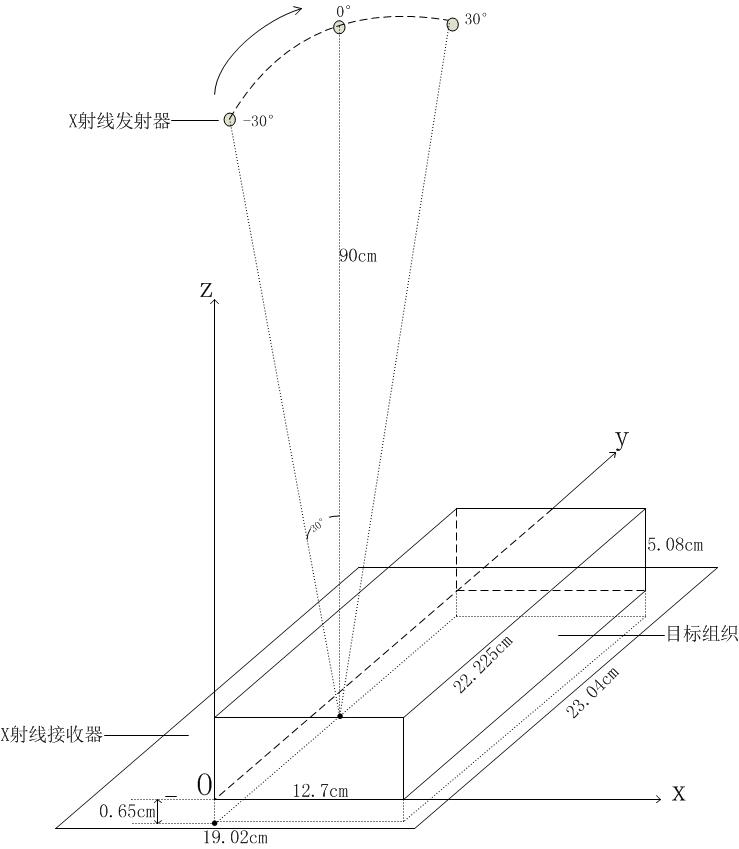
\includegraphics[width=0.8\textwidth]{figure/model1}
\caption{有限角度CT重建的探测模型}\label{fig:model1}
\end{figure}
在整个探测系统中,正下方是一面探测平面,宽度为$19.2cm$,长度为$23.4cm$,其分辨率为$1902*2304$在接收板宽的正中,长边的边缘处,
以之为原点建立一个图中所示的直角坐标系,$x$轴沿宽边方向,$y$轴沿长边方向,而$z$轴则垂直向上。物块与
探测器的边缘相平行的放置,且距离探测平面有一定的高度,高度为$0.65cm$。物块的$xoz$
平面距离探测的边缘约为$0.4cm$\footnote{这个距离未标识出。另外,由于被探测物体内部
的肿块不在边缘处,所以后期重建的范围小于物体大小,因此这个距离并不重要。}。在探测器中央
上方垂直$90cm$处有一个X-射线发射管,它可以以它正下方与探测平面的交点为圆心
进行小角度旋转,正负角度均为$30^\centerdot$。探测管以它为中心向下方发射锥形的光束,
穿过被测物体并照射在探测平面上,探测平面接收到X-射线,并将吸收量记录传递。探测管每
隔$3^\centerdot$向探测平面发射一次X射线,一共采集$21$组投影数据。
\subsection{物体模型}
物块整体是一个长方体,大小约为$12.7cm*23.4cm*5.08cm$。
\begin{figure}[h!]
\center
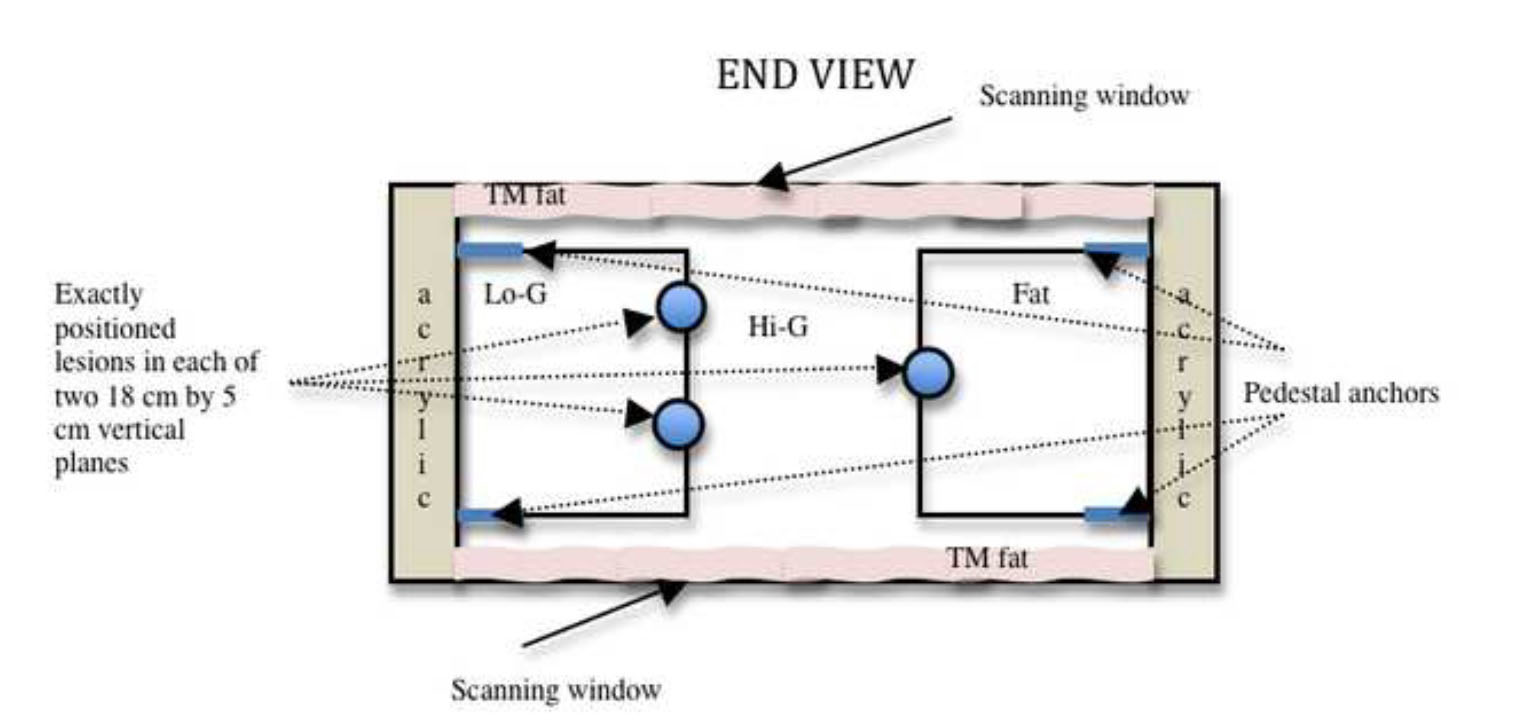
\includegraphics[width=0.8\textwidth]{figure/object/front}
\caption{探测物块正视图}\label{fig:objfront}
\end{figure}
\begin{figure}[h!]
\center
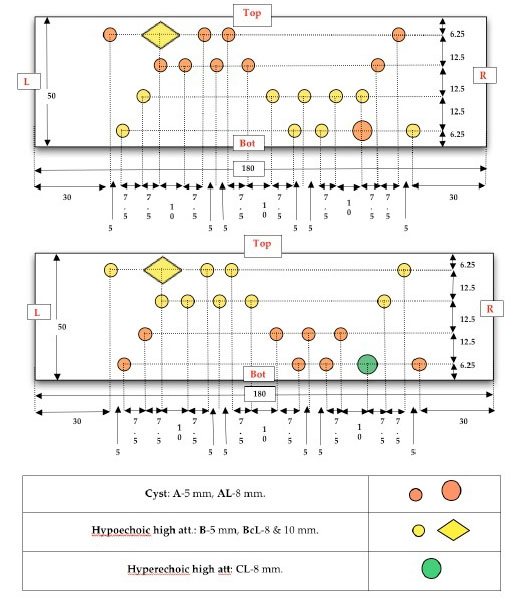
\includegraphics[width=0.8\textwidth]{figure/object/side}
\caption{探测物块侧视图}\label{fig:objside}
\end{figure}
\begin{figure}[h!]
\center
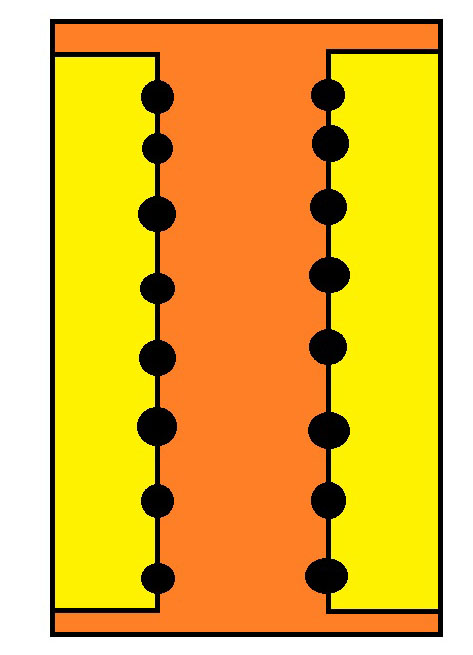
\includegraphics[width=0.8\textwidth]{figure/object/top}
\caption{探测物块俯视图}\label{fig:objtop}
\end{figure}
图\ref{fig:objfront}为物块的正视透视图,图\ref{fig:objside}为
物块的侧视透视图,而\ref{fig:objtop}则为物块的俯视透视图。
可以看到,物块内部有大小不等的圆形以及菱形肿块。CT重建的主要目的
就是恢复重建这些肿块。此外,物块整体本身由不同的物质
分块组成,而在CT重建中应该能清楚看到不同物质的交界面。

\subsection{超声数据}
三维超声图像重建数据是一种对CT重建的补充与辅助数据。在使用超声
探测时,超声以平行于$y$轴的方向向物块发射并探测,由此得到相应的重建
数据。由于超声探测自身的特点以及它的探测方向特点,它的重建数据在$z$方向分辨率
较高,边缘清晰且伪影较轻,恰恰可以补充CT有限角度重建的不足。在本文要探究的模型中,将直接使用已经重建完成
的超声数据。

\section{解析类算法}
正如章节\ref{sec:current}所描述,CT重建主要基于两类方法,第一类便是解析类算法。这类算法主要基于
傅里叶切片定理(The Fourier Slice Theorem)\cite{bracewell1986fourier},是目前CT成像方面的主流算法。
\subsection{雷登变换(Radon Transform)}
雷登变换是将不同角度发射线在途径路径上线性积分后成为的一个和角度与位置相关
的函数。其基本表达式如下:
\begin{equation*}
p_\phi(r)=\int_{\mathcal{L}(r,\phi)}f(x,y)dl
\end{equation*}
其中
\begin{equation*}
\mathcal{L}(r,\phi)=\{(x,y)\in R^2:x\cos\phi+y\sin\phi=r\}
\end{equation*}
这类解析方法要研究的主要目的就是如何从雷登变换函数$p$中将原图像$f(x,y)$所重建出来。

\subsection{傅里叶切片定理}
CT重建解析类方法的基础就是傅里叶切片定理,它的表述如下:
令$P_\phi(\nu)$表示雷登变换后函数$p_\phi(r)$的傅里叶变换,也就是
\begin{equation*}
P_\phi(\nu)=\int^\infty_{-\infty}p_phi(r)e^{-i2\pi \nu r}dr
\end{equation*}
令$F(u,v)$表示原图函数$f(x,y)$的二维傅里叶变换,也就是
\begin{equation*}
F(u,v)=\int^\infty_{-\infty}\int^\infty_{-\infty}f(x,y)e^{-i2\pi(ux+vy}dxdy
\end{equation*}
结合上述式子,可以得到傅里叶切片定理:
\begin{equation*}
P_\phi(\nu)=F(\nu\cos\phi,\nu\sin\phi),\qquad \forall\nu\in R,\quad\forall\phi\in R
\end{equation*}
在上式中$F(\nu\cos\phi,\nu\sin\phi)$代表的是$F(u,v)$的极坐标形式。

通过傅里叶切片定理,我们发现在傅里叶变换的情况下,雷登变换形式函数和原图的函数
被联系在了一起,这也意味着我们可以通过该联系从雷登变换函数中恢复原图的函数。

\subsection{直接傅里叶重建(Direct Fourier reconstruction)}
根据傅里叶切片定理,可以很自然得到重建的方法\cite{de1968reconstruction}。
\begin{algo}
直接傅里叶重建算法
\begin{enumerate}
\item{将每个$p_\phi()$函数傅里叶变换获得$P\phi()$}
\item{使用傅里叶切片定理的关系产生原图的二维傅里叶极坐标表示,也就是
\begin{equation*}
F(\rho,\phi)=P_\phi(\rho)
\end{equation*}}
\item{将极坐标表示下的$F(\rho,\phi)$转化为直角坐标系下的$F(u,v)$。这个过程需要谨慎考虑插值问题}
\item{通过傅里叶反变换从$F(u,v)$中获得$f(x,y)$}
\end{enumerate}
\end{algo}

\subsection{反向投影-滤波方法(The backproject-filter method)}
该方法首先将函数$p_\phi()$反向积分成模糊掉的原图函数,再将之傅里叶变换成频域图像,
通过补偿的方法消除频域上的模糊值,再重新反投影。\cite{smith1973image}

其算法概述如下:
\begin{algo}
反向投影-滤波方法
\begin{enumerate}
\item{使用带权重的反向投影将函数$p_\phi$变为模糊的原函数$f_b(x,y)$}
\item{使用傅里叶变换将$f_b(x,y)$获得$F_b(u,v)$}
\item{在频域使用带角度的锥形滤波
\begin{equation*}
\hat{F}(u,v)=\cfrac{\sqrt{u^2+v^2}}{w(\angle_\pi(u,v))}F_b(u,v)
\end{equation*}
其中滤波器的具体形式见文献\cite{smith1973image},它的频率相应为锥形,因此成为锥形滤波器}
\item{恢复$f(x,y)$的直流分量,最后得到$\hat{F}(u,v)$}
\item{通过傅里叶反变换将$\hat{F}(u,v)$变为$\hat{f}(x,y)$}
\end{enumerate}
\end{algo}

\subsection{滤波—反向投影方法(The filter-backproject method)}
之前的反向投影-滤波方法是先将未滤波的雷登变换函数
反向投影产生一个模糊的原图像函数,再将之在频域进行滤波。
步骤总结如下:
\begin{equation*}
f(x,y)\rightarrow\boxed{\text{投影}}
\rightarrow p_\varphi(r)\rightarrow\boxed{\text{反向投影}}
\rightarrow f_b(x,y)\rightarrow\boxed{\text{锥形滤波}}\rightarrow
f(x,y)
\end{equation*}
因为头两个操作是线性与移位操作,因此可以将它移动到后面,可以得到
\begin{equation*}
f(x,y)\rightarrow\boxed{\text{锥形滤波}}\rightarrow
\breve{f}(x,y)\rightarrow\boxed{\text{投影}}
\rightarrow \breve{p}_\varphi(r)\rightarrow\boxed{\text{反向投影}}
f(x,y)
\end{equation*}
由于$f(x,y)$是未知的,上述的方法直接实施是不可行的,但是
\begin{equation*}
\breve{p}_\varphi(r)\xlongleftrightarrow{\text{FT}}{}
\breve{P}_\varphi(\nu)=\breve{F}(\rho,\varphi)\arrowvert_{\rho=\nu}
=|\rho|F(\rho,\varphi)\arrowvert_{\rho=\nu}=|\nu|F(\nu,\varphi)=|\nu|P_\varphi(\nu)
\end{equation*}
因此,我们可以对$p_\varphi(r)$进行滤波,因为形状,我们称之为斜坡滤波(Ramp filters)。
综合上面所述,滤波-反向投影方法可以描述如下。
\begin{algo}
滤波—反向投影方法
\begin{enumerate}
\item{对于每个投影角度$\varphi$,计算对应的$p_\varphi$的一维傅里叶变换得到、
对应的$P_\varphi(\nu)$}
\item{把$P_\varphi(\nu)$乘上$|\nu|$(斜坡滤波)}
\item{对于每个$\varphi$,计算$|\nu|P_\varphi(\nu)$的傅里叶变换得到被滤波
的投影$\breve{p}_\varphi(r)$。在实际操作中,这个过程通常由FFT来完成}
\item{由于斜坡滤波缺失直流分量,因此要把投影补上缺失的直流分量}
\item{对$\{\breve{p}_\varphi(r)\}$进行反向投影:
\begin{equation*}
\breve{f}(x,y)=\int^\pi_0\breve{p}_\varphi(x\cos\varphi+y\sin\varphi)d\varphi
\end{equation*}}
\end{enumerate}
\end{algo}
\section{代数重建算法}
在代数重建类算法中,主要有两种代表性算法,一种是由Gordon, Bender和Herman
在\cite{gordon1970algebraic}中所提出的Algebric Reconstruction Technique(ART)
算法,这是此类算法中最早的。另外还有由Anderson和Kak在\cite{andersen1984simultaneous}
中所提出的Simultaneous Algebraic Reconstruction Technique(SART)算法。作为本文
的基础,将在后小节中重点讲述上述算法。

\subsection{代数表示概述}
为了能使用代数重建方法,我们首先需要将投影的过程以代数的方式所表示出来。
我们知道,图像本是连续的信息,我们为了能在计算机中存储、表示,将之离散化
为一个一个像素点。
通常,一束射线通过被测物体\footnote{为了简化问题,这里用平面来表示},可以用一个线性
方程来表示出来。当有多束光线经过时,可以以如下方式表示
\begin{align*}
w_{11}x_1+w_{12}x_2+w_{13}x_3+\cdots+w_{1N}x_N &= b_1\\
w_{21}x_1+w_{22}x_2+w_{23}x_3+\cdots+w_{2N}x_N &= b_2\\
\cdots\\
w_{M1}x_1+w_{M2}x_2+w_{M3}x_3+\cdots+w_{MN}x_N &= b_M\\
\end{align*}
在这里,$w$是一束光线在每个点的权重,$x$是被测图像的每个点。而$N$为像素点总数,$M$
为光线总数。上述方程也可以写成矩阵形式
\begin{equation*}
\bm{W}\x=\bb
\end{equation*}

而现在的问题是,权重矩阵$\bm{W}$应该如何确定。在\cite{gordon1970algebraic}中,将每个像素定位
网状格子,如果光线通过这个像素所代表的格子,则把相应的权重置为$1$,否则为$0$。在\cite{shepp1974fourier}
中,则通过光束与经过的格子所相交面积比例来确定权重。一种Digital Differential 
Analyzer 算法\cite{foley1990computer}也被用于提高权重计算的速度。当然,上述的
方法都是基于像素的格形表示。如图\ref{fig:nest}所示。
\begin{figure}[!h]\label{fig:nest}
\center
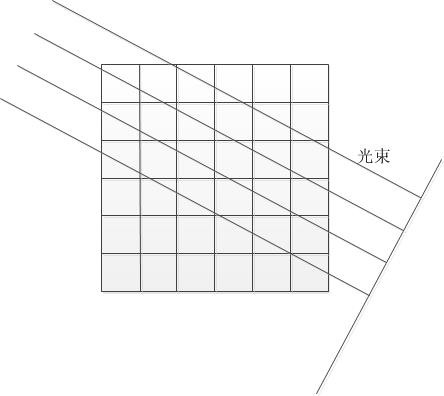
\includegraphics[width=0.6\textwidth]{figure/ART/zuobiao.jpg}
\caption{格形表示示意图}
\end{figure}

\subsection{投影矩阵计算}\label{sec:sartA}
在本文所采用的方法中,将使用文献\cite{andersen1984simultaneous}所使用的代数表示方法。

对于一幅图像$f(x,y)$,为了将其离散化,使用$N$个基图像$\{b_i(x,y)\}$,则存在
一组实数$g_1,g_2,\cdots,g_N$,有
\begin{equation}
f(x,y)\simeq\breve{f}(x,y)\equiv\sum^N_{i=1}g_ib_i(x,y)
\end{equation}
$\breve{f}(x,y)$是图像的近似。以$r_j(x,y)=0$表示第$j$个射线的方程,则这个射线
的投影矩阵可以表示为
\begin{equation}
p_j=R_jf(x,y)=\int^\infty_{-\infty}\int^\infty_{-\infty}f(x,y)\delta(r_j(x,y))dxdy
\end{equation}
假设$f(x,y)$是一个平方可积函数。对于这个有限维度的模型,投影算子的线性可以
得到
\begin{equation}
R_j\breve{f}(x,y)=\sum^N_{i=1}g_iR_ib_i(x,y)
\end{equation}
而在实际的使用时,会将$R_jb_j(x,y)$替换成近似的数值$a_{ij}$来实现计算。
因此,可以有
\begin{equation}
p_j=R_jf(x,y)\simeq R_j\breve{f}(x,y)=\sum^N_{i=1}g_iR_jb_i(x,y)\simeq\sum^N_{i=1}g_ia_{ij}
\end{equation}
如果用$e_j$来表示近似所产生的误差,则有
\begin{equation*}
p_j=\sum^N_{i=1}g_ia_{ij}+e_j
\end{equation*}

在选择基准图像时,选择的方式正如上文所说,将图像分割成$N$个等大小的像素格。
如前所述,这里积分表示的选择有很多。如果不考虑光束的宽度,则需要考虑光束与
每个像素格子所相交的长度。而如果给光束加上一个有限的长度,则要考虑光束与像素
格子所相交的面积,而投影矩阵的元素因此也表示为了面积。

为了降低椒盐噪声,许多研究者都采用了这样一种方式来进行代数重建:即对投影的每个
像素(每个视点),都考虑一条光束\cite{smith1977practical}。这样做的话,被测图像
的每个像素点都会与探测光束相交多次,因此其噪声就可以被平均而降低。其中,方程数
大约四倍于被探测图像的像素点数\cite{herman2009fundamentals}。当然,计算量也会提升。

为了得到一个精确的投影描述,对于光束所途径的点,可以采用二次插值的方式来确定。这种
方式也相对比较简单\cite{herman1976iterative}\cite{andersen1982digital}。每一个
要计算的点的值由它四周的四个采样点的二次插值来决定。这样,虽然图像本身是离散,
这种二次插值允许我们从一种连续的角度来进行代数表示。

下面用这种方式来给出$a_{ij}$。考虑一条通过被探测图像的光束$R_j$,将它从通过探测图像
开始,平均等分为$M_j$个点,用$\Delta s$来表示等分的长度,$\breve{f}(s_{jm})$则
表示等分点上的灰度值,见图\ref{fig:sart1}。可以得到积分式为
\begin{figure}[!h]\label{fig:sart1}
\center
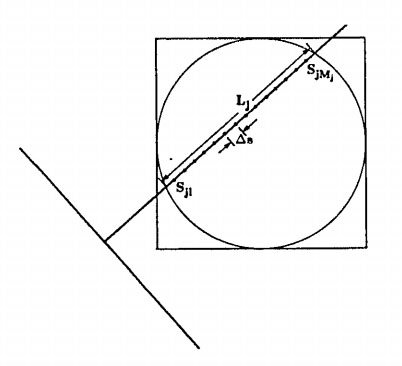
\includegraphics[width=0.6\textwidth]{figure/ART/sart1}
\caption{投影计算示意图}
\end{figure}
\begin{equation}\label{eq:pj1}
p_j\simeq\sum^{M_j}_{m=1}\breve{f}(s_{jm})\Delta s
\end{equation}
$\breve{f}(s_{jm})$的值,正如之前所述,由它周围的四个点来插值决定,可以写成
\begin{equation}\label{eq:pj2}
\breve{f}(s_{jm})=\sum^N_{i=1}d_{ijm}g_i,\qquad \text{for}m=1,2,\cdots,M_j
\end{equation}
数值$d$代表的是插值系数。把方程\eqref{eq:pj1}和方程\eqref{eq:pj2}相结合,
就可以得到沿着光束的积分$p_j$,它是图像采样$g_i$的线性函数形式:
\begin{equation}
\begin{split}
p_j&=\sum^{M_j}_{m=1}\sum^N_{i=1}d_{ijm}g_i\Delta s \\
&=\sum^N_{i=1}\sum^{M_j}_{m=1}d_{ijm}g_i\Delta s \\
&=\sum^N_{i=1}a_{ij}g_i
\end{split}
\end{equation}
所以,$a_ij$就可以表示为光束所经过的每一个计算点的插值系数的
线性组合形式:
\begin{equation}\label{eq:computea}
a_{ij}=\sum^{M_j}_{m=1}d_{ijm}\Delta s
\end{equation}
在这里,$a_{ij}$需要注意的是,它的尺度大小需要符合真实的物理模型。也就是说,需要
调整权重以满足$\sum^N_{i=1}a_{ij}$与光束与物体相交的长度$L_j$相等。

此外就是等分步长$\Delta s$。它的大小很重要,如果设置太小,则会加重计算的负担,
如果设置太大,则可能产生较大噪声且不够精确。因此需要在其中折中取值。
在\cite{andersen1984simultaneous}中提到,一般$\Delta s$取值为采样步长一半时
可以在计算量和精确度之间取得一个良好的效果。

\subsection{ART算法}
按照上述的坐标描述,ART算法的迭代式子可以表示为\cite{gordon1974tutorial}
\cite{gordon1970algebraic}\cite{herman1973art}:
\begin{equation}
\bg\upp{k+1}=\bg\upp{k}+\ba_j\cfrac{p_j-\ba^T_j\bg\upp{k}}{\ba^T_j\ba_j}
\end{equation}
其中$\ba_j$为投影矩阵中的第$j$列。可以看到这是一种迭代计算,
对每一条光束,
都会更新一次$\bg$,且$\bg$的初始值都设置为$0$。当所有光线全部被计算
过一次之后,就完成了一次计算循环。
\subsection{SART算法}
SART算法在ART算法的基础上,对其迭代公式进行了一定的改进。其算法如下\cite{andersen1984simultaneous}:
\begin{equation}
g_i\upp{k+1}=g_i\upp{k}+\cfrac{\sum_j\bigl[a_{ij}\cfrac{p_j-\ba^T_j\bg\upp{k}}{\sum^N_{i=1}a_{ij}}\bigr]}{\sum_ja_{ij}}
\end{equation}
在ART算法中,分别对每条光束进行一次迭代和更新,而在
SART算法之中,则一次迭代要考虑所有的光束。可以看到,对于第$i$个像素,
其迭代项被以$j$进行迭代,其分子$\sum^N_{i=1}$代表了第$j$条光束的长度。
而ART算法中的分母也被改成了$\sum^N_{i=1}a_{ij}$,这个项在
同步重建过程中用于平衡图像数值。
\section{算法选择}
对于存在的两大类算法,其各有优势。代数算法相比之于解析类算法,
存在的缺点是计算量很大。然而,它在数据不足时的重建是可行的,
比解析类算法拥有更少的噪声。

考虑到本文需要解决的问题是通过先验知识提高小角度CT成像的质量,
代数类算法就成为自然而然的选择。对于本文问题,它有如下优势:
\begin{enumerate}
\item 小角度CT本身就是一种数据缺失的图像重建
,而使用代数重建算法可以在这种情况下较好重建数据
\item 在代数重建的过程中,由于其是
迭代项使用的形式,更容易加入先验知识优化重建过程
\end{enumerate}
\section{小结}
在本章节中,先给出了需要解决的问题模型。其中包括被探测的物体的模型,
探测系统的模型,以及先验知识的情况。

鉴于需要解决的问题是一个CT重建问题,自然需要讨论可行的解决方案。所以接下来
先讨论了比较流行的解析类算法,即基于傅里叶切片理论的几种经典算法。

接下来,又讨论了相对应用较少的代数类算法。列出了这类算法的数学系统,以及两个
经典算法ART和SART的基本形式。

在最后的分析讨论中,本文认为,采用代数重建类算法对于本文需要解决的
问题是最可行的,因此,将基于代数类算法来解决本文的问题。在后文中,
将详细讨论本文所提出的重建算法。


\chapter{基于SART的优化算法}
\section{算法概述}
本文在SART算法的基础上,改进了一种优化算法,该算法可以把超声成像的信息融合到重建的过程中,从而在重建中可以
引导重建图像的生成,使得重建以一种合理的方式融合X射线tomography与超声成像的优势,由此来弥补小角度成像所造成
的信息缺失。下面是本文所提出的优化算法的基本框架。
\begin{algo}\label{mysart}
基于SART的优化算法
\begin{algorithmic}[1]
\STATE
Initialize $\x^{(0)} \leftarrow \bm{0}$,$t\leftarrow \bm{0}$
\REPEAT
\STATE
$\bL(\x^{(t)}) \leftarrow  \V^{-1}\A^T\W(\bb-\A\x^{(t)})$ \\
$\bP(\x^{(t)}) \leftarrow \B^{T}(\bh-\B\x^{(t)})$ \\    %水平
$\bQ(\x^{(t)}) \leftarrow \C^{T}(\bv-\C\x^{(t)})$         %垂直
\STATE
$\x^{(t+1)}\leftarrow \omega\bL(\x^{(t)}) + \lambda\bP(\x^{(t)}) + \xi\bQ(\x^{(t)})    $
\UNTIL{convergence}
\end{algorithmic}
\end{algo}

在算法\ref{mysart}中,$\x$代表的是所重建的数据,为一维向量,是将立体的物体模型以确定方向的坐标延伸而成。
$\bL(x^{(k)})$,分别是tomo约束的迭代增量,而$\bP(x^{(k)})$和$ \bQ(x^{(k)})$是超声数据的信息
的迭代增量\footnote{在算法中可以增加多个先验知识,在本文中我们使用了两个信息,分别为超声数据的不同方向所提取的,
具体见章节\ref{sec:mysart},后同。}。矩阵$\A$是在Tomography中X射线的投影矩阵,$\V$是对角矩阵,它的对角元素
是$V_{j,j}=A_{+,j}$,$\W$也是对角矩阵,其元素为$V_{j,j}=A_{i,+}$,$\B,\C$是提取超声信息所用的矩阵,
$\bh,\bv$则是超声信息中所提取出来信息,也是一维向量。
$\omega,\lambda_h,\lambda_v$
分别是三者的迭代步进参数。关于该算法的细节在接下来的章节中进一步描述。


\section{算法细节描述}
\subsection{使用梯度信息}\label{sec:mysart}
在前所述的研究工作中,我们发现:
\begin{enumerate}
    \item 由于X射线tomography是小角度重建的原因,本质上信息是缺失的。在我们的模型中所直接看到的情况就是肿块
    在垂直方向上的大小变化不清晰,并没有清楚的变化边缘,而是呈现逐渐模糊掉的形式。这点是超声数据可以弥补的,
    它在肿块边界的变化上有明显的优势。
    \item 超声重建的探测方向与x射线tomography的探测方向并不相同。x射线tomography的探测方向是在被测物体上方往下
    放射,而放射管在一个小角度里转动。相比之下超声重建的探测方向是被测物体的边上以垂直于tomography的方向发射的,
    由此可以知道两者在物体不同部分的信息也并不相同。特别是在经过了两者数据的配准之后,在沿超声探测方向上实际上已经
    有了插值数据,而这些数据实际上如果完全应用于重建是不合理的。
    \item 物体内不同材料对X射线和超声的吸收特性是不一样的,甚至可能会呈现相反的趋势。
    \item 超声重建后的数据存在着不小的噪声。
\end{enumerate}
在上述讨论中,我们可以发现,直接应用超声数据到重建中是不合理的,因为超声数据有许多冗余的信息会误导到tomo重建。同时,
我们可以发现,我们所需要的是超声重建数据的边缘信息。超声数据对肿块清晰的边缘可以弥补tomography重建中肿块边缘信息的缺失,
同时即使材料对X射线和超声的吸收特性不同,不同材料之间的边缘信息也是一致的。因此,如果能有效利用边缘信息,我们便可以把
超声信息的优势加入到数据重建中。

为了利用边缘信息,将使用图像的梯度作为要提取的信息。在图~\ref{fig:model}中,我们看到超声是沿着$y$轴进行探测,由此超声重建数据
在$x,z$方向上的梯度具有较多的有用信息。特别是在$z$方向上的梯度,包含有肿块在$z$方向上的变化信息,这可以对tomogarphy重建的肿块在
这个方向上边缘变化不明显的问题做一个比较好的补偿。

在算法~\ref{mysart}中,有$\bh,\bv$实际上就是超声提取的梯度信息,这个是直接对超声重建的数据取梯度并经过一定的处理完成的一维向量
\footnote{直接得到的梯度图像包含有大量的噪声,还不能直接使用,需要经过处理,见章节\ref{sec:gradprocess}}。
而$\B,\C $则是对图像取梯度的矩阵算子。
\clearpage

\subsection{算法展开}\label{sec:algodetail}
将算法~\ref{mysart}根据前述章节内容展开,我们将得到每一次迭代的过程如下:
\begin{align}
 L_k(x_i) &= \cfrac{1}{A_{+,k}}\sum^N_{i=1}\cfrac{A_{i,k}}{A_{i,+}}\bigl(b_i-\bar{b_i}(x\upp{t})\bigr) \label{eq:L} \\
P_k(x^{(t)}) &= \begin{cases}
                            -(2x_k\upp{t} - x_{k+mn}\upp{t} - x_{k-mn}\upp{t} - h_k + h_{k-mn}) & mn \le k \le N-mn \\
                            -(x_k\upp{t} - x_{k+mn}\upp{t} - h_k) &  k\le mn \\
                            -(x_{k-mn}\upp{t} - x_{k}\upp{t} - h_{k-mn}) &  N-mn \le k \le N
                        \end{cases}  \label{eq:P} \\
Q_k(x^{(t)}) &= \begin{cases}
                            -(2x_k\upp{t} - x_{k+n}\upp{t} - x_{k-n}\upp{t} - v_k + v_{k-mn}) & k \notin [ imn-n+1, imn+n]
                            \\ &i = 0,1,2\hdots\\
                            -(x_k\upp{t} - x_{k+n}\upp{t} - v_k) & k \in \left[imn+1,imn+n\right] \\ &i = 0,1,2\hdots\\
                            -(x_{k-n}\upp{t} - x_{k}\upp{t} - v_{k-n}) &  k \in [imn-n+1,imn] \\ &i= 1,2,3 \hdots
                        \end{cases} \label{eq:Q} \\
x_k^{(t+1)}&= x_k\upp{t} + \omega L_k(x^{(t)}) + \lambda P_k(x^{(t)}) + \xi Q_k(x^{(t)}) \label{eq:all}
\end{align}
其中$m,n$分别是被测立方物体底面的两边长度,$m$为$x$方向上的边长,$n$为$y$方向上的边长。$N$为物体所有的像素点数。

上述就是基于SART的优化算法采用两个方向的梯度信息的结果。方程\eqref{eq:L}, \eqref{eq:P}, \eqref{eq:Q}分别给出了三项的展开结果,其中方程
\eqref{eq:P}, \eqref{eq:Q}是已经将梯度运算矩阵$\B,\C$代入的结果。而方程
\eqref{eq:all}将三项的迭代项通过步进参数调整后加到$\x$上进行迭代。可以看到,该算法的展开结果与SART算法相比,
是在SART的基础上增加了两项超声梯度信息项,这两项超声梯度信息项将超声的梯度信息融合到了重建中。在后面的部分中我们可以看到,这种
算法可以使得被重建的物体将在满足tomograph投影约束。
\begin{equation*}
\A\x = \bb
\end{equation*}
与两个梯度约束
\begin{align*}
\B\x &= \bh \\
\C\x &= \bv
\end{align*}
中取得全局最优化的结果。



\section{基于SART优化算法的理论证明}
\subsection{优化目标的建立}\label{sec:optobj}
在章节\ref{sec:algodetail}中,提到了被重建的物体需要满足tomograph投影约束与两个梯度约束,在这三个约束中间取到最优化。事实上,基于约束
的优化也正是SART算法的本质所在。我们知道,在tomography的投影探测中,X射线穿过物体,并被沿途的被测物体物质进行一定量的吸收,最后发射
到传感器上,传感器检测到射线的吸收量。由此,这个吸收量其实就是被物体该射线所穿过的每个像素沿着探测射线进行累积(积分)的量。由于我们
需要采用数值方法计算,物体的像素被我们离散,所以这个吸收量实际上就是射线途径的物体像素的累积和。对于每一条射线,我们都
可以用一个相应的矩阵来代表它的路径。它实际上就是与物体等大小的一个矩阵。我们将物体的像素写成一位列向量$\x$的形式后,该矩阵实际上就变成
了与之等长的一个行向量。将所有探测光束所代表的横向量进行排列以后,实际上就得到了我们的投影约束矩阵$\A$。而相应的得到的投影数据也
写成一个一维列向量的形式$\bb$。因此,我们得到了方程
\begin{equation}
\A\x = \bb \label{eq:tomocon}
\end{equation}
此外,在章节\ref{sec:mysart}中提到,我们要将超声数据的梯度信息融合到重建中。实际上,就是要使得重建的物体的固定方向的梯度上要与超声数据
对应方向的梯度相接近。考虑到SART算法实际上是解决这样一个优化问题:
\begin{equation}
\x = \argmin_{\x\in R^N}\W\norm{\A\x-\bb}^2 \label{eq:sartopt}
\end{equation}
方程\eqref{eq:sartopt}的优化其实是一个带权的最小平方误差优化,权$\W$ 是因为SART的形式需要加上。这个优化,实际上就是在寻找一个值$\x$,它能使得$\A\x$与得到的投影数据 $\bb$的相差最小。在本文中,将它的范数定为损失函数。
注意范数函数都为凸函数,因此这是一个凸优化。
将梯度的约束加上,我们就得到
\begin{equation}
\x = \argmin_{\x\in R^N}\W\norm{\A\x-\bb}^2 +\norm{\B\x-\bh}^2+\norm{\C\x-\bv}^2 \notag
\end{equation}
实际上,这样并不是最合理的,因为这样可能会使得最后的数据偏向tomo的约束方向或者偏向梯度约束方向。注意我们是要使得重建的数据在一定程度上
被引向梯度约束,因此,可以在上面的优化目标中增加参数$c,d$用来控制各个约束对数据的影响程度,这些参数可以在实验中确定一个最佳值,因此
,方程变为
\begin{equation}
\x = \argmin_{\x\in R^N}\W\norm{\A\x-\bb}^2 +c\norm{\B\x-\bh}^2+d\norm{\C\x-\bv}^2 \qquad c>0,d>0 \label{eq:mysartopt}
\end{equation}
注意在方程\eqref{eq:mysartopt}中,它由于是多个范数的非负权重和,因此它还是一个凸函数\cite{boyd2004convex},这仍然是一个凸优化。而为了解决
这个优化问题,我们将使用梯度下降算法\cite{nesterov2003}。



\subsection{梯度下降算法}\label{sec:graddescent}
我们知道,负梯度$-f'(x)$是函数下降最快的方向。因此,如果要求目标最小值的话,
可以将被优化目标往它的负梯度方向每次步进一些,就能到达一个局部最小值,
梯度下降算法框架如下:
\begin{algo}
对于一个可微的优化目标 $f(x)$
\begin{algorithmic}[1]
\STATE
选择一个$x_{0}\in R^n$
\STATE
迭代\\
$x_{k+1}=x_{k}-h_kf'(x_{k}),\qquad k=0,1,\hdots$
\end{algorithmic}
\end{algo}
其中$h_k$被称为step size,步进大小。它的值可以挑选合适的,比如
\begin{align*}
h_k &= h>0,\quad h\text{为常数}\\
h_k &= \cfrac{h}{\sqrt{k+1}}
\end{align*}
在\cite{nesterov2003}中给出了梯度下降算法的性能分析。定义
$C^{k,p}_L(Q)$是一族$k$阶可微函数,其第$p$阶导数在$Q$上满足Lipschitz
连续,也就是
\begin{equation*}
\norm{f\upp{p}(x)-f\upp{p}(y)}\le L\norm{x-y}\qquad \text{对于所有的} x,y\in Q
\end{equation*}
考虑这个优化问题
\begin{equation}\label{eq:gdopt}
\min_{x\in R^n}f(x)
\end{equation}
其中$f(x)\in C^{1,1}_L(R^n)$,我们假设$f(x)$在$R^n$上有下界,且步进参数
为常数。由$y=x-hf'(x)$,从上述假设里首先我们可以得出
\begin{equation}
\begin{split} \label{eq:une}
f(y) &\le f(x) + \inner{f'(x),y-x}+\frac{L}{2}\norm{y-x}^2  \\
     &= f(x)-h\norm{f'(x)}^2+\frac{h^2}{2}L\norm{f'(x)}^2 \\
     &= f(x)-h(1-\frac{h}{2}L)\norm{f'(x)}^2
\end{split}
\end{equation}
因此,为了估计最佳的下降大小,我们需要解这个一维问题:
\begin{equation*}
\Delta (h)=-h(1-\frac{h}{2}L)\rightarrow\min_h
\end{equation*}
取这个函数的导数,我们可以得到$\Delta '(h)=hL-1=0$,因此,解
是$h^\star=\frac{1}{L}$,同时这也是$\Delta(h)$的最小值。

因此,前式变为
\begin{equation*}
f(y)\le f(x)-\cfrac{1}{2L}\norm{f'(x)}^2
\end{equation*}
当考虑之前的迭代策略$x_{k+1}=x_k-h_kf'(x_k)$,$h_k=h$代入,有:
\begin{equation*}
f(x_k)-f(x_{k+1})\ge h(1-\cfrac{1}{2}Lh)\norm{f'(x_k)}^2
\end{equation*}
现在考虑一般情况下的情况。由上面的集中类型我们可以得到
\begin{equation}
f(x_k)-f(x_{k+1})\ge \cfrac{\omega}{L}\norm{f'(x_k)}^2
\end{equation}
其中$\omega$是一个正常数。

将上面的式子以$k=0,\hdots,N$累加起来,可以得到
\begin{equation}
\cfrac{\omega}{L}\sum^N_{k=0}\norm{f'(x_k)}^2\le f(x_0)-f(x_N)
\le f(x_0)-f^\star
\end{equation}
其中$f^\star$是对问题\eqref{eq:gdopt}的最优化值。因此,
由上式我们可以得出
\begin{equation*}
\norm{f'(x_k)}\rightarrow 0 \qquad k\rightarrow \infty
\end{equation*}
也就是说,被优化函数的梯度$f'(x)$可以在一定次数的迭代之后趋向于$0$。定义收敛序列
\begin{equation*}
g^\star_N=\min_{0\le k\le N}g_k
\end{equation*}
其中$g_k=\norm{f'(x_k)}^2$。于是,可以得到下述不等式:
\begin{equation}
g^\star_N \le \cfrac{1}{\sqrt{N+1}}[\cfrac{1}{\omega}L(f(x_0)-f^\star)]^{1/2}
\end{equation}
上市右边项提示了$g^\star_N$与$N$的关系。

在\cite{nesterov2003}中还对梯度下降算法的收敛性进行了分析。有定理
\begin{thm}\label{thm:graddecent}
令函数$f(x)$满足如下的假设:
\begin{enumerate}
\item{$f\in C^{2,2}_M(R^n)$}
\item{存在函数$f$的局部最小值,且在这个点上它的Hessian是正定的}
\item{存在一些边界$0<l\le L<\infty$,对于在点$x^\star$的Hessian来说,有
\begin{equation*}
lI_n\le f''(x^\star)\le LI_n
\end{equation*}}
\end{enumerate}
且令$x_0$足够接近局部最小值:
\begin{equation*}
r_0=\norm{x_0-x^\star}<\bar{r}=\cfrac{2l}{M}
\end{equation*}
于是使用合适的步进值的梯度下降方法可以以如下的速率收敛:
\begin{equation*}
\norm{x_k-x^\star}\le \cfrac{\bar{r}r_0}{\bar{r}-r_0}(1-\cfrac{l}{L+l})^k
\end{equation*}
\end{thm}
也就是说,梯度下降算法是线性收敛的。在章节\ref{eq:optobj}中提到,我们的目标函数为多个范数非负权相加的形式。由于范数
函数本身是凸的,所以这个非负权和的形式也是凸的。我们知道,凸函数有一个特点,是有唯一全局最小点。因此,采用梯度下降
算法所收敛到的局部最小点就是全局最小点。同时,我们也在定理\ref{thm:graddecent}中看到梯度下降算法具有优良的收敛性,
因此使用梯度下降算法解这个优化问题是合理的。另外,在后文中我们会看到SART算法本身的形式也是能利用梯度下降算法来解释,
这也更进一步增加了使用梯度下降算法的合理性。



\subsection{优化问题求解}
接下来将采用梯度下降算法来推导出算法\ref{mysart}。重新将优化目标\ref{eq:mysartopt}写在这里
\begin{equation}
\min_{\x\in R^N}\W\norm{\A\x-\bb}^2 +c\norm{\B\x-\bh}^2+d\norm{\C\x-\bv}^2 \qquad c>0,d>0
\end{equation}
我们令
\begin{equation*}
\bF(\x) = \W\norm{\A\x-\bb}^2 +c\norm{\B\x-\bh}^2+d\norm{\C\x-\bv}^2
\end{equation*}
它是一个连续可微的函数,所以我们求它的梯度
\begin{equation*}
\nabla \bF(\x) = 2(\A^T\W(\A\x-\bb)+c\B^T(\B\x-\bh)+d\C^T(\C\x-\bv))
\end{equation*}
使用梯度下降,我们有
\begin{equation}\label{eq:gradout}
\begin{split}
\x\upp{t+1}&=\x\upp{t}-\cfrac{\omega}{2}\V^{-1}\nabla F(\x\upp{t})\\
&=\x\upp{t} + \omega\V^{-1}\A^T\W(\bb-\A\x\upp{k})
           + c\omega\V^{-1}\B^T(\bh-\B\x)
           + d\omega\V^{-1}\C^T(\bv-\C\x)
\end{split}
\end{equation}\label{eq:gradfinal}
令$\lambda = c\omega\V^{-1},\xi = d\omega\V^{-1}$
于是方程\eqref{eq:gradout}变为
\begin{equation}\label{eq:gradout2}
\x\upp{t+1}= \x\upp{t} + \omega\V^{-1}\A^T\W(\bb-\A\x\upp{k})
           + \lambda \B^T(\bh-\B\x\upp{k})
           + \xi \C^T(\bv-\C\x\upp{k})
\end{equation}
可以发现,方程\eqref{eq:gradfinal}其实就是算法\ref{mysart}
的迭代过程。在其中,为了能得到SART基础项的正确形式,设置步进常数为$\tfrac{\omega}{2}\V^{-1}$,
这样可以使得正常的SART可以不被破坏\footnote{SART的设置本身具有良好的收敛性,这点我们在后文中会提到},而
在上面的最后一步中,我们将$\omega\V^{-1}$和梯度相自带的
常数$c,d$(可以是矩阵)一起合并成一个简单的常数项$\lambda ,\xi$,这个步骤实际上就是一定程度
上把梯度项的迭代和tomogaphy的投影项的迭代过程分离开来。如果常数项选择不当的话,轻的后果是可能使得其中一些项的作用超过其它项,而
严重的话则从定理
\ref{thm:graddecent}中,我们可以知道,会使得
迭代过程不再收敛。可以发现,我们的优化目标中含有矩阵$\A$,它是一个复杂的大矩阵(tomography投影矩阵),
此外,还带有权矩阵$\W$,这与梯度项所带的梯度计算矩阵$\B,\C$的数量级往往并不一样,所以优化目标将变的较为复杂,
直接采用解析的方法计算合理的步进常数项是难以实现的,因此,将在实验中确定合理的参数项。

下面将推导出该算法的展开具体展开形式。


\subsection{梯度矩阵计算}
首先要给出计算梯度的计算。先分析$\x$的排列。我们知道,它是将三维的物体数据伸展成一维的。物体的模型
示意见图\ref{fig:model2}。
\begin{figure}[ht]
\center
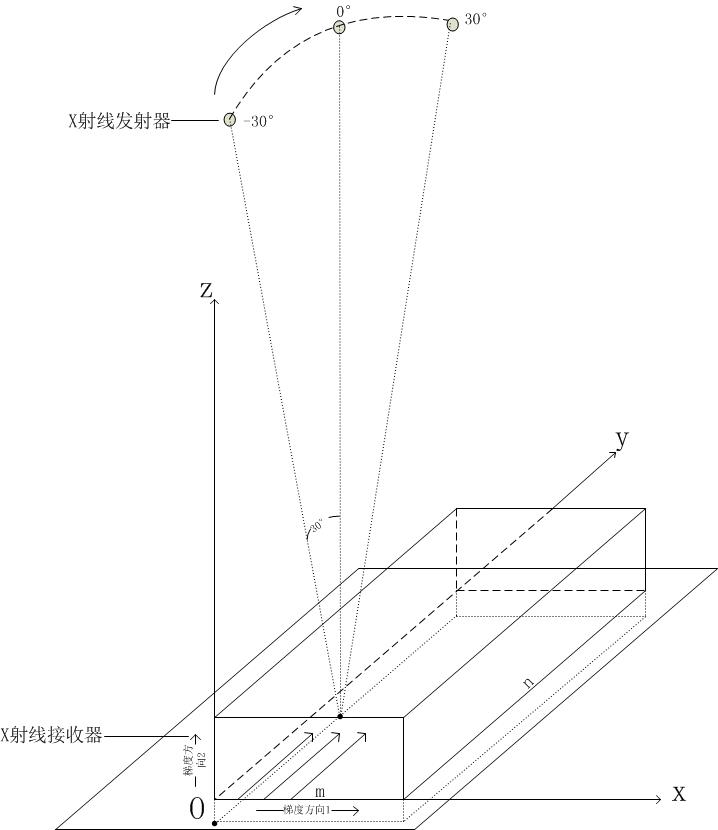
\includegraphics[width=0.8\textwidth]{figure/model2.jpg}
\caption{探测物体模型}\label{fig:modle2}
\end{figure}
在图中,探测物体在$x$方向的边长为$m$,在$y$方向的边长为$n$。注意图中沿$y$轴的三根箭头,三维物体的像素索引顺序是依照此箭头进行的。也就是说,索引顺序的第一级顺序是$y$轴正方向顺序,第二级顺序是$x$
轴正方向顺序,第三级顺序是$z$轴正方向顺序。对于一个在物体中的坐标标号为$I_{xyz}$的的像素点而言,它在$\x$中的坐标索引$x_i$计算方式如下:
\begin{equation}\label{eq:indexconvert}
x_i = I_{xyz}\qquad \text{当} i = mnz+nx+y
\end{equation}
从取梯度的角度考虑,我们不选择超声探测平行的方向梯度信息,这是因为探测本身的积分特性,会使得在这个方向上相对被模糊,也就是
梯度信息不如与超声探测方向相垂直的方向。由于超声影像的探测方向是沿着$y$轴正方向照射,我们选择在$x$,$z$两个方向的梯度信息。

首先处理沿着$z$轴的梯度方向。要计算沿着该方向的梯度。实际上就是对于所计算出来的梯度$grad$,这样的:
\begin{equation}\label{eq:grad_z1}
grad_{xyz} = I_{xyz}-I_{xy(z+1)}
\end{equation}
方程\eqref{eq:grad_z1}没有涉及到最后一个平面的问题。一般来说,梯度的边缘并不是十分重要,因此,为了方便未来的计算,将边缘处补$0$。
由式\eqref{eq:indexconvert}可以得到:
\begin{equation}\label{eq:grad_z2}
g_i = \begin{cases}
        x_{i} - x_{i+mn} & i \le N-mn \\
        0   & i \in [N-mn+1,N]
        \end{cases}
\end{equation}
对于式\eqref{eq:grad_z2},可以写成矩阵形式:
\begin{equation*}
\bg = \C \x
\end{equation*}
其中矩阵$\C$如下:
\begin{equation*}
\C = \begin{pmatrix}
1 & 0 & 0 & 0 & \cdots &-1 & 0 &0 &0 &\cdots \\
0 & 1 & 0 & 0 &\cdots &0 & -1 &0 &0 &\cdots \\
\hdotsfor[3]{3}& 1& \cdots &\hdotsfor[3]{3}&-1&\cdots \\
0 & 0 & 0 & \hdotsfor[3]{5}&0&0 \\
\hdotsfor[3]{10}\\
\hdotsfor[3]{10}\\
0 & 0 & \ddots & 0 & \cdots & 0 & 0 & \ddots & 0& \cdots
\end{pmatrix}
\end{equation*}
或者可以写成
\begin{equation*}
\C = \begin{pmatrix}
\bI &  -\bI & \0 & \0 & \0 \cdots \\
\0 & \bI &  -\bI & \0 & \0 \cdots \\
\0 & \0  & \ddots & \ddots & \0 & \cdots \\
\hdotsfor[3]{7} \\
\0 & \0 & \0 &\cdots & \0 & \0 &\0 \cdots
\end{pmatrix}
\end{equation*}
其中,$\bI$是一个大小为$mn * mn$的单位矩阵,而$bm 0$ 则是大小为$mn * mn$的零矩阵。
于是我们可以得到关于$\C$ 矩阵的归纳式:
\begin{equation}\label{eq:C}
C_{ij} = \begin{cases}
1 & i = j,\quad i\le N-mn \\
-1 & i = j- mn,\quad i\le N- mn \\
0 & \text{其它}
\end{cases}
\end{equation}

接下来是$\B$矩阵的推导。对于$\B$,其求梯度方向是沿着$x$轴方向。同样的,为了未来计算方便,在边缘处补$0$。
这个边缘也就是物体沿着$x$轴的最外侧。类似于$\C$,可以得到:
\begin{equation*}
\B = \begin{pmatrix}
1 & 0 & 0 & 0 & \cdots &-1 & 0 &0 &0 &\cdots \\
0 & 1 & 0 & 0 &\cdots &0 & -1 &0 &0 &\cdots \\
0 & 0 & \ddots & 0 & \cdots & 0 & 0 & \ddots & 0& \cdots \\
\hdotsfor[3]{3}& 1& \cdots &\hdotsfor[3]{3}&-1&\cdots \\
0 & 0 & 0 & \hdotsfor[3]{5}&0&0 \\
\hdotsfor[3]{10}\\
\hdotsfor[3]{10}
\end{pmatrix}
\end{equation*}
为了方便描述,也可以写成矩阵形式:
\begin{equation*}
\B = \begin{pmatrix}
\tilde{\bI} &  -\tilde{\bI} & \0 & \0 & \0 \cdots \\
\0 & \tilde{\bI} &  -\tilde{\bI} & \0 & \0 \cdots \\
\0 & \0  & \ddots & \ddots & \0 & \cdots \\
\hdotsfor[3]{7} \\
\0 & \0 & \0 &\cdots & \0 & \0 &\0 \cdots
\end{pmatrix}
\end{equation*}
其中,$\tilde{\bI}$是一个大小为$n * n$的矩阵,描述如下:
\begin{equation*}
\tilde{\bI} = \begin{pmatrix}
1 & 0 & 0 & \cdots &\cdots & \cdots\\
0 & 1 & 0 & \cdots &\cdots & \cdots\\
 & &\ddots & \\
& & & \cdots& 1 & 0 \\
0 & \cdots & \cdots & \cdots & \cdots & 0
\end{pmatrix}
\end{equation*}
而$\bm 0$ 则是大小为$n * n$的零矩阵。于是$\B$可以写成归纳形式如下:
\begin{equation}\label{eq:B}
B_{ij} = \begin{cases}
1 & i=j, \quad i \notin [kmn-n+1,kmn] \\
-1 & i = j-n \quad i \notin [kmn-n+1,kmn] \\
0 & \text{其它}
\end{cases}
\end{equation}

现在,矩阵$\B$和$\C$ 都已经得到了,我们需要对式子\eqref{eq:gradout2}作进一步展开,并得到可以计算的最终结果。

\subsection{展开结果的获得}
考虑式子
\begin{equation*}
\B^T(\bh-\B\x)
\end{equation*}
先将内部展开,根据$\B$ 的定义,可以得到:
\begin{equation*}
\begin{split}
(\bh-\B\x)_i &= -(\sum_{j=1}^{N}B_{ij}x_j - h_i)\\
             & = \begin{cases}
             -(x_i -x_{i+n} -h_i)  & i \notin [kmn-n+1,kmn]\\
             0  & \text{其它} \\
             \end{cases} \\
             & = T_i
\end{split}
\end{equation*}
再展开的式子的外层,有
\begin{equation*}
(\B^T(\bh-\B\x))_j = \sum_{j=1}^{N}\B_{ij}T_i \\
\end{equation*}
考虑到$\B$ 定义,即式子\eqref{eq:B},上式可以进一步展开为
\begin{equation*}
\sum_{j=1}^{N}\B_{ij}T_i =  \begin{cases}
T_j -T_{j-n} & j\notin [kmn-n+1,kmn+n]\\
T_j  & j \in [kmn+1,kmn+n] \\
-T_{j-n} & j \in [kmn-n+1,kmn]
\end{cases}
\end{equation*}
将上述式子进一步展开,就得到
\begin{equation} \label{eq:Bout}
(\B^T(\bh-\B\x))_j = \begin{cases}
-(2x_j -x_{j+n} -x_{j-n} -h_j + h_{j-n}) & j\notin [kmn-n+1,kmn+n]\\
-(x_j-x_{j+n}-h_j) & j \in [kmn+1,kmn+n] \\
(x_{j-n}-x_j-h_{j-n} & j \in [kmn-n+1,kmn]
\end{cases}
\end{equation}

接下来考虑式子
\begin{equation*}
\C^T(\bh-\C\x)
\end{equation*}
先将内部展开,根据$\C $的定义,可以得到:
\begin{equation*}
\begin{split}
(\bv-\C\x)_i &= -(\sum_{j=1}^{N}C_{ij}x_j - v_i)\\
             & = \begin{cases}
             -(x_i -x_{i+mn} -v_i)  & i \notin [N-mn+1,kmn]\\
             0  & \text{其它} \\
             \end{cases} \\
             & = Y_i
\end{split}
\end{equation*}
再展开的式子的外层,有
\begin{equation*}
(\C^T(\bv-\C\x))_j = \sum_{j=1}^{N}\C_{ij}Y_i \\
\end{equation*}
考虑到$\C$ 定义,即式子\eqref{eq:C},上式可以进一步展开为
\begin{equation*}
\sum_{j=1}^{N}\C_{ij}Y_i =  \begin{cases}
Y_j -Y_{j-n} & j\in [mn,N-mn]\\
Y_j  & j \in [1,mn] \\
-Y_{j-mn} & j \in [N-mn,N]
\end{cases}
\end{equation*}
将上述式子进一步展开,就得到
\begin{equation} \label{eq:Cout}
\C^T(\bh-\C\x))_j = \begin{cases}
-(2x_j -x_{j+mn} -x_{j-mn} -v_j + v_{j-n}) & j\in [mn,N-mn]\\
-(x_j-x_{j+mn}-v_j) & j \in [1,mn] \\
(x_{j-mn}-x_j-v_{j-mn} & j \in [N-mn,N]
\end{cases}
\end{equation}

对于式子\eqref{eq:gradout2}中的第一项,我们可以直接展开得到:
\begin{equation}\label{eq:Aout}
(\omega\V^{-1}\A^T\W(\bb-\A\x))_j = \cfrac{\omega}{A_{+,j}}
\sum_{i=1}^M\cfrac{A_{i,j}}{A_{i,+}}(b_i-\bar{b}_i(x))
\end{equation}
在上式中
\begin{align*}
A_{i,+}=\sum_{j=1}^N{A_{i,j}} \\
A_{+,j}=\sum_{i=1}^M{A_{i,j}} \\
\bar{b}_i(x)=(\A\x)_i
\end{align*}
其中$N,M$分别表示矩阵$A$的横、纵长度。矩阵$A$是投影矩阵,将在具体问题中获得,
在章节\ref{sec:obtainA}中会详细介绍。

于是,将式\eqref{eq:Aout}式\eqref{eq:Bout}以及式\eqref{eq:Cout}代入到式\eqref{eq:gradout2}中,
就可以得到我们算法的完整展开形式了。



\section{基于SART算法的收敛性}

在章节\ref{sec:graddescent}中,已经提到了梯度下降算法的收敛性在一定的条件下(该条件一般都满足)是线性时间的。
而SART算法本身就是一种梯度下降算法,加在其前面的是相应的矩阵项$\V^{-1}$,其实是相当于在最小平方误差中的每一个维度
分别添加了一个相应的参数。而对于SART迭代项的收敛性,在论文\cite{jiang2003convergence}中对其做了详细的总结与证明。

\subsection{SART算法的收敛性证明}
\cite{jiang2003convergence}中中先证明了SART算法解的存在性。
令$N(A)$是矩阵$\A$的零空间,则根据正交分解理论有:
\begin{equation*}
\R^N=N(A)\oplus N(A)^\perp
\end{equation*}
其中$N(A)^\perp$表示$N(A)$的正交补子空间,令$R(\A^T)$表示矩阵$\A^T$的值域,
所以,可以知道$N(A)^\perp=R(\A^T)$

令
\begin{equation*}
L(x)=\sum_{i=1}^M\cfrac{1}{A_{i,+}}(b_i-\bar{b}_i(x))^2=\norm{\bb-\A\x}^2_W
\end{equation*}
其中$\norm{\bb-\A\x}^2_W = \W\norm{\bb-\A\x}^2$,它的梯度表示为:
\begin{equation*}
\nabla L(\x)=-2\A^T\W(\bb-\A\x)
\end{equation*}
而所有$L$的最小化点要满足
\begin{equation}\label{eq:normaleq}
\A^T\W\A\x=\A^T\W\bb
\end{equation}
因为$\inner{\A^T\W\A\x,\x}=\norm{\A\x}^2_W$,因此可以得到$N(A^TWA)=N(A)$。
且因为$\A^T\W\bb\in R(\A^T) = N(A)^\perp$,\ref{eq:normaleq}存在解。

令S为\eqref{eq:normaleq}的解集。
则由于$L(x)$是在$\x$上的凸函数,\eqref{eq:normaleq}
的解也是$L$的最小化点,反之亦然。所以$S$也是$L$在$\R^N$上的最小化点集。

接下\cite{jiang2003convergence}中证明了SART算法的收敛性问题。其中有:
\begin{equation*}
L(x\upp({x}))-L(x\upp{k})\le -\alpha\norm{x\upp{k+1}-x\upp{k}}^2_V
\end{equation*}
其中$\alpha = 2/\omega -1 > 0$。又有下述推论:
\begin{enumerate}
\item{$\{L(x\upp{k})\}^\infty_{k=0}$有界。}
\item{$L(x\upp{k+1})\le L(x\upp{k})$}
\item{\begin{equation*}
L(x\upp{k+1})+\alpha\sum^k_{j=0}\norm{x\upp{j+1}-x\upp{j}}^2_V\le L(x_0)
\end{equation*}}
\item{$\sum^\infty_{j=0}\norm{x\upp{j+1}-x\upp{j}}^2_V$收敛}
\item{\begin{equation*}
\norm{x\upp{k+1}-x\upp{k}}\rightarrow 0,\text{对于}k\rightarrow \infty
\end{equation*}}
\end{enumerate}


考虑希尔伯特空间$\chi$,通过正交分解,我们有
\begin{equation*}
\chi = N(A)\oplus N(A)^{\perp V}
\end{equation*}
其中$N(A)^{\perp V}$表示在$\chi$中的子空间$N(A)$的正交补。
因为$S$也是在$\chi$中的闭集,它一定包含唯一的元素$x^\ast$能产生最小的
$V$-范数。很显然,$x^\ast\in N(A)^{\perp V}$。

通过方程\eqref{eq:normaleq},SART可以被写成
\begin{equation*}
x\upp{k+1}-x^\ast = x\upp{k}-x^\ast + \omega V^{-1}A^TWA(x^\ast-x\upp{k})
\end{equation*}
令$z\upp{k}=x\upp{k}-x^\ast$,我们有
\begin{equation*}
z\upp{k+1}=z\upp{k}-\omega V^{-1}A^TWAz\upp{k}
\end{equation*}
通过一定的数学处理,可以得到
\begin{equation*}
\norm{z\upp{k+1}}^2_V=\norm{z\upp{k}}^2_V
+\norm{z\upp{k}-z\upp{k+1}}^2_V-2\omega \norm{Az\upp{k}}^2_W
\end{equation*}
与
\begin{equation*}
\norm{z\upp{k+1}}^2_V\le \norm{z\upp{k}}^2_V
+\norm{z\upp{k}-z\upp{k+1}}^2_V
\end{equation*}

此外,序列$\{z\upp{k}\}$是收敛的。令$r_k=\norm{z\upp{k}}^2_V$,则序列
$\{r_k\}$也是收敛的,也就是说,$\lim_{k\rightarrow \infty}r_k$存在。
最后,可以得到由SART所得到的序列$x\upp{k}$收敛于$P[x_0]+x^\ast$,只要
$\omega\in (0,2)$。
 
\subsection{基于SART算法的收敛性说明}
上述的证明已经说明了SART算法是收敛的。接下来考虑基于SART的优化算法的收敛性。
式子\eqref{eq:gradout2}中,我们可以看到,除了SART算法项以外,还多出了两项属于
梯度约束的迭代计算项。但是可以发现,在我们的图像梯度信息项实际上是
以与梯度下降算法完全相同的形式存在于式子中,不像SART算法项一样还存在多余的矩阵参数。
前文提到,梯度下降的算法在一定条件下是收敛的。当然,当这些项叠加在一起的时候,我们
无法完全确定迭代是否收敛\footnote{事实上在实验中,参数选择不当时确实出现迭代不收敛的现象}。
因此我们才增加了相应的尺度参数$\lambda,\xi$来控制后面的梯度约束项。在$\lambda=0,\xi=0$
的情况下,后两项梯度控制项消失,而只剩下SART项,这时候该算法就退化成了SART算法,而SART算法是收敛的,
但是$\lambda,\xi$过于小的时候,超声数据的梯度信息就无法影响到重建。因此,我们需要控制$\lambda,\xi$的大小,
使这个迭代能够收敛,同时又能正确将梯度信息融合到重建之中。这两个参数的大小,就将在后面的
实验中来确定。


\section{小结}
在本章中,给出了本文最主要的内容,也是本文的创新点:即基于SART的优化算法。首先给出了基于SART优化算法的
的框架形式,并讨论了如何将算法应用到所要解决的问题。分析遇到的问题所在,需要将超声数据的有用
信息融合到重建之中,针对超声数据的特点,本文提出应当利用它的梯度信息,这样可以避免掉材料对超声和X射线的
不同吸收特性问题,也可以避免掉一部分的噪声影响。

接下来,给出了利用梯度信息的算法展开形式。在之后的章节中,
对基于SART的优化算法理论上的合理性给予了证明。首先是将要解决的问题写成一个优化问题的形式。对于这个优化问题,
指出它是多项范数平方的非负权和,这是一个凸函数。因此该优化是一个凸优化,对于凸优化,它具有唯一的全局最优解,
并且它的局部最优就是全局最优。因此,采用了梯度下降算法来解决这个优化问题。对于梯度下降,我们引用文献
说明了它的性能。接下来,将采用优化算法的迭代形式写出。为了展开迭代形式,先分析并计算了两个方向的梯度矩阵,并将
矩阵代入相应的迭代项中展开获得了具体的展开形式。而SART的迭代项展开后就是原SART算法的形式,将几个项的展开形式叠加起来,
就得到了可以具体实现的算法展开形式。

在完成了证明之后,又说明了基于SART的优化算法的收敛性。本文引用相关文献,
给出了SART算法的收敛性分析,并通过SART算法的收敛性,对基于SART的优化算法的收敛性进行了说明。采用参数控制的形式,
使得算法可以在接近SART算法的基础上,能够收敛到一个合理的解上。

至此,本算法的理论部分已经说明完毕。接下来要讨论具体的实现过程。


\chapter{超声数据的配准}
\section{简介}
在本实验中,所获得的Tomography相应的数据,与超声数据并不是匹配的
%%以下是超声数据和tomography数据的说明

从上面的看

\chapter{算法的验证实验}
\section{梯度叠加项的可行性}
在章节\ref{sec:mysart}和\ref{sec:algodetail}中,给出并展开了基于SART的优化算法。在具体实现整体算法之前,先要
对梯度信息融合的效果作一个预估。
\subsection{实验计算公式}
我们忽略TOMO重建的项,只考虑如下的迭代计算:
\begin{align*}
P_k(x^{(t)}) &= \begin{cases}
                            -(2x_k\upp{t} - x_{k+mn}\upp{t} - x_{k-mn}\upp{t} - h_k + h_{k-mn}) & mn \le k \le N-mn \\
                            -(x_k\upp{t} - x_{k+mn}\upp{t} - h_k) &  k\le mn \\
                            -(x_{k-mn}\upp{t} - x_{k}\upp{t} - h_{k-mn}) &  N-mn \le k \le N
                        \end{cases}   \\
Q_k(x^{(t)}) &= \begin{cases}
                            -(2x_k\upp{t} - x_{k+n}\upp{t} - x_{k-n}\upp{t} - v_k + v_{k-mn}) & k \notin [ imn-n+1, imn+n]
                            \\ &i = 0,1,2\hdots\\
                            -(x_k\upp{t} - x_{k+n}\upp{t} - v_k) & k \in \left[imn+1,imn+n\right] \\ &i = 0,1,2\hdots\\
                            -(x_{k-n}\upp{t} - x_{k}\upp{t} - v_{k-n}) &  k \in [imn-n+1,imn] \\ &i= 1,2,3 \hdots
                        \end{cases}  \\
x_k^{(t+1)}&= x_k\upp{t} + \lambda P_k(x^{(t)}) + \xi Q_k(x^{(t)})
\end{align*}
在matlab中实现相应的算法。为了方便起见,我们采用二维图像作为模型而不是三维的物理。在二维的情况下,
两个梯度方向分别选择$x,y$方向梯度,于是上述的算法式子变成二维的形式:
\begin{align*}
P_{ij}(x^{(t)}) &= \begin{cases}
                            -(2x_{ij}\upp{t} - x_{(i+1)j}\upp{t} - x_{{i-1}j}\upp{t} - h_{ij} + h_{(i-1)j}) & 2 \le i \le Y-1 \\
                            -(x_{ij}\upp{t} - x_{(i+1)j}\upp{t} - h_{ij}) &  i = 1 \\
                            -(x_{(i-1)j}\upp{t} - x_{ij}\upp{t} - h_{(i-1)j}) &  i = Y
                        \end{cases}   \\
Q_{ij}(x^{(t)}) &= \begin{cases}
                            -(2x_{ij}\upp{t} - x_{i(j+1)}\upp{t} - x_{i(j-1)}\upp{t} - v_{ij} + v_{i(j-1)}) & 2 \le j \le X-1\\
                            -(x_{ij}\upp{t} - x_{i(j+1)}\upp{t} - v_{ij}) &  j = 1 \\
                            -(x_{i(j-1)}\upp{t} - x_{ij}\upp{t} - v_{i(j-1)}) &  j = X
                        \end{cases}  \\
x_{ij}^{(t+1)}&= x_k\upp{t} + \lambda P_k(x^{(t)}) + \xi Q_k(x^{(t)})
\end{align*}
因为是在matlab中实现,因此重新将索引改成了二维的形式,即$i,j$,其中$X,Y$分别为$x,y$方向的图像边长。

\subsection{实验条件}
在实验中,采用的原图为和融合的梯度图大小均为$256*256$。原图的所有像素点全部初始化为
$0$,我们的梯度图采用一个简单的正方形作为模板。图\ref{fig:I1}为原图,图\ref{fig:p1}为所要融合的图像。
图\ref{fig:px1},\ref{fig:py1}分别为所要融合的梯度信息图像的$x,y$方向信息。
\begin{figure}[h!]
\center
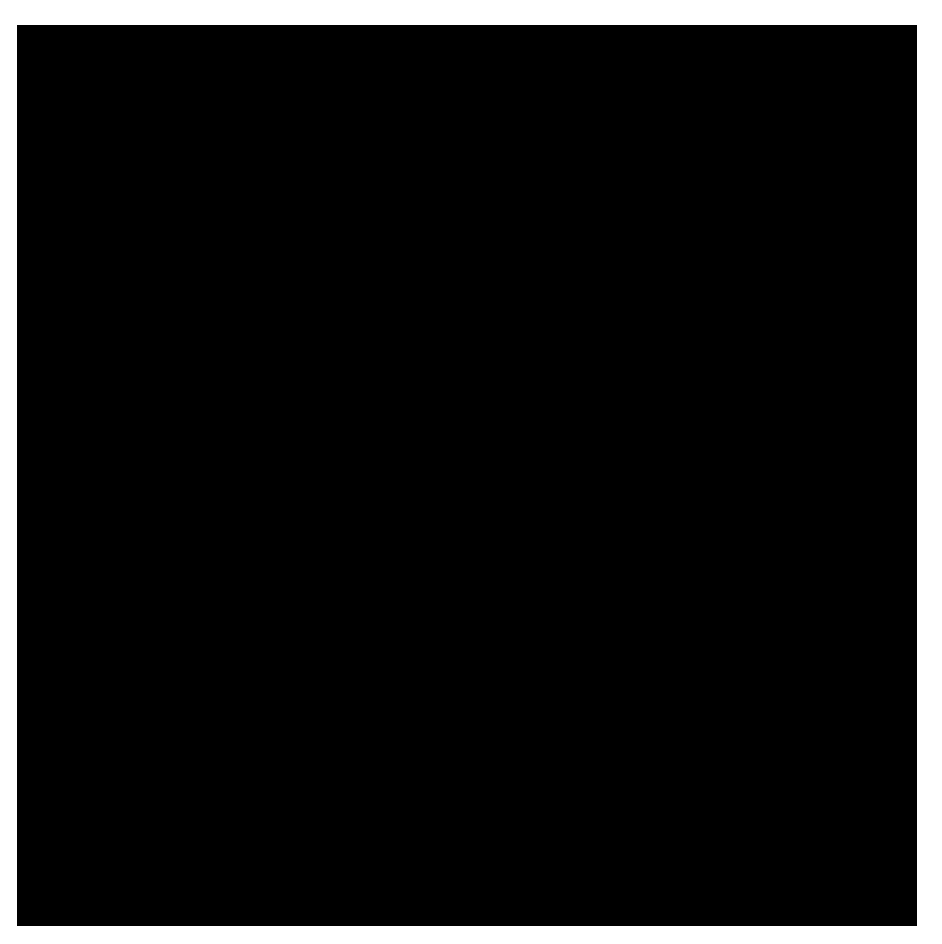
\includegraphics[width=0.5\textwidth]{figure/gradtest/I1}
\caption{原图}\label{fig:I1}
\end{figure}
\begin{figure}[h!]
\center
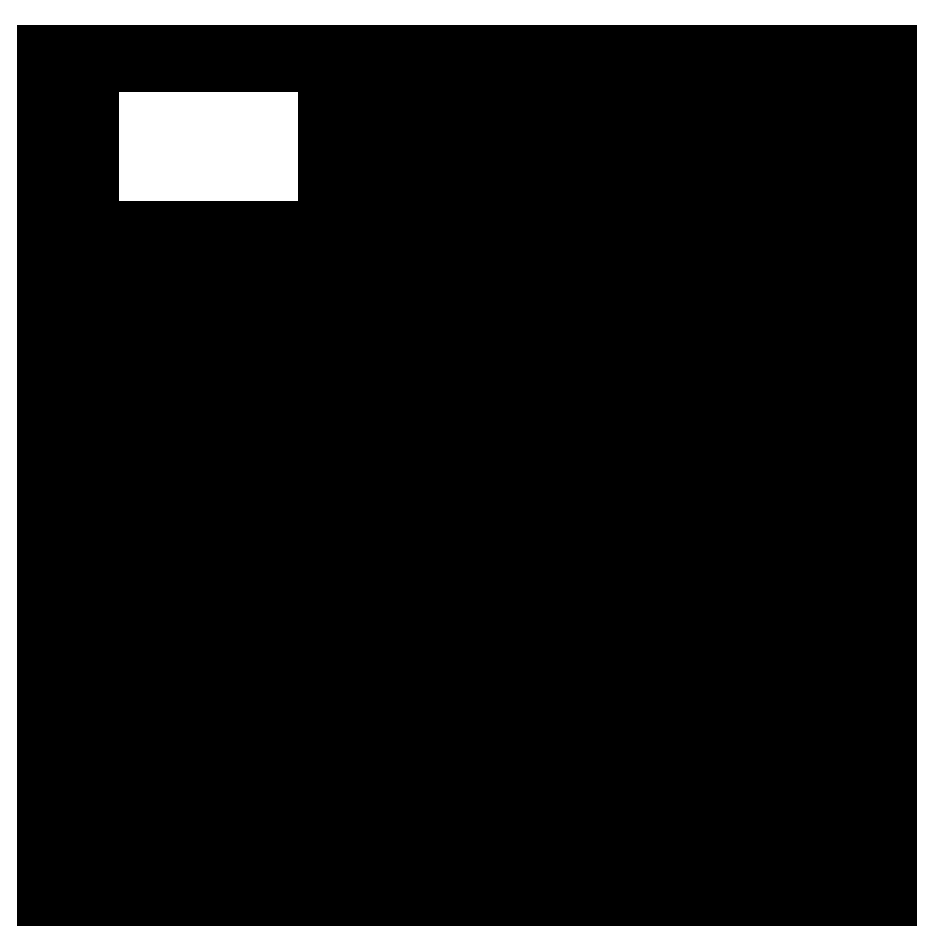
\includegraphics[width=0.5\textwidth]{figure/gradtest/p1}
\caption{梯度模板}\label{fig:p1}
\end{figure}
\begin{figure}[h!]
\center
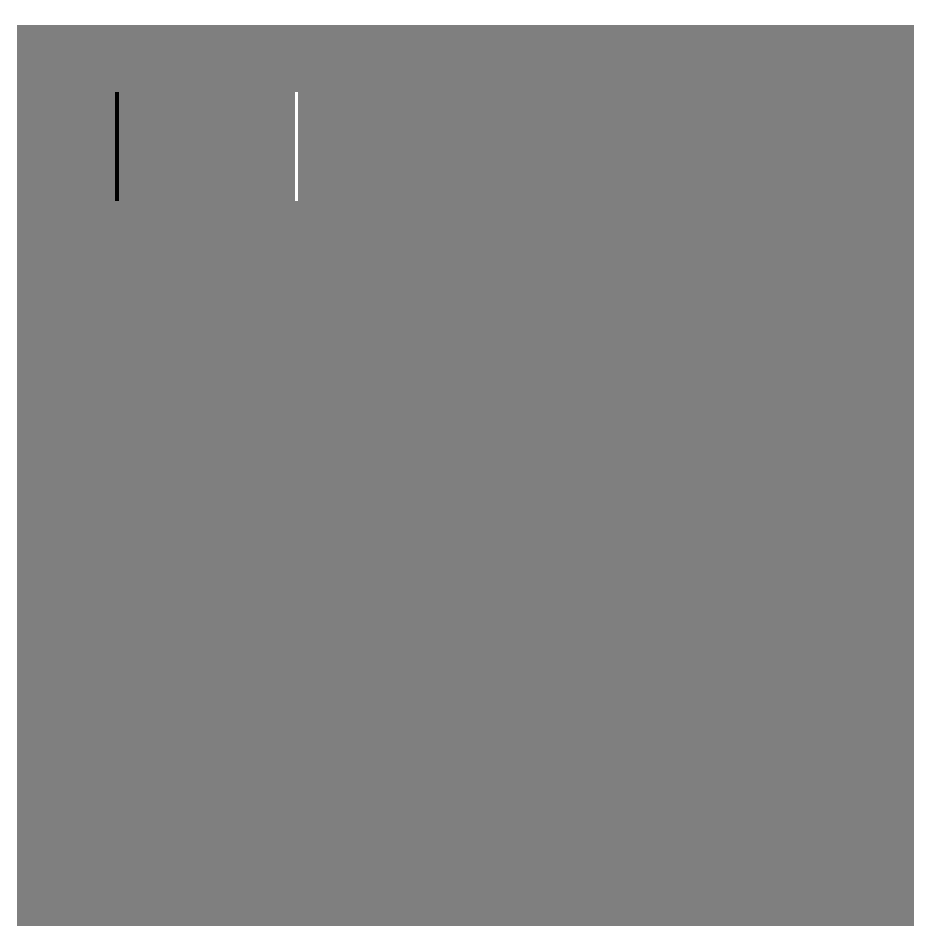
\includegraphics[width=0.5\textwidth]{figure/gradtest/px1}
\caption{梯度模板 x方向梯度}\label{fig:px1}
\end{figure}
\begin{figure}[h!]
\center
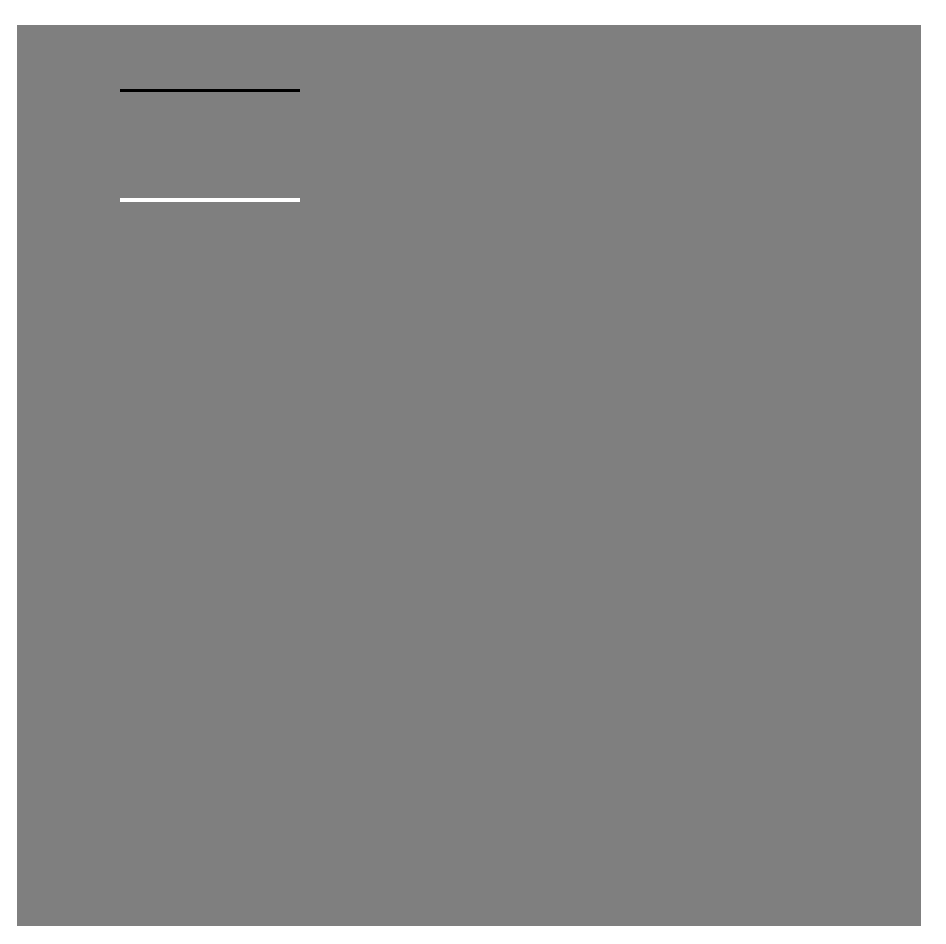
\includegraphics[width=0.5\textwidth]{figure/gradtest/py1}
\caption{梯度模板 y方向梯度}\label{fig:py1}
\end{figure}

\FloatBarrier
\subsection{不收敛的结果}
首先,在实验中发现,$\lambda$和$\xi$对是否收敛起到至关重要的作用。当$\lambda$和$\xi$都取$1$的时候,
得到的结果是不收敛的的。图\ref{fig:Iout1}是得到的结果图像。可以看到得到的是一些有规律的纹路图,但是
本身没有任何意义。再来看它的$x,y$方向的梯度图,即图\ref{fig:Ioutx1}和图\ref{fig:Iouty1}。
\begin{figure}[h!]
\center
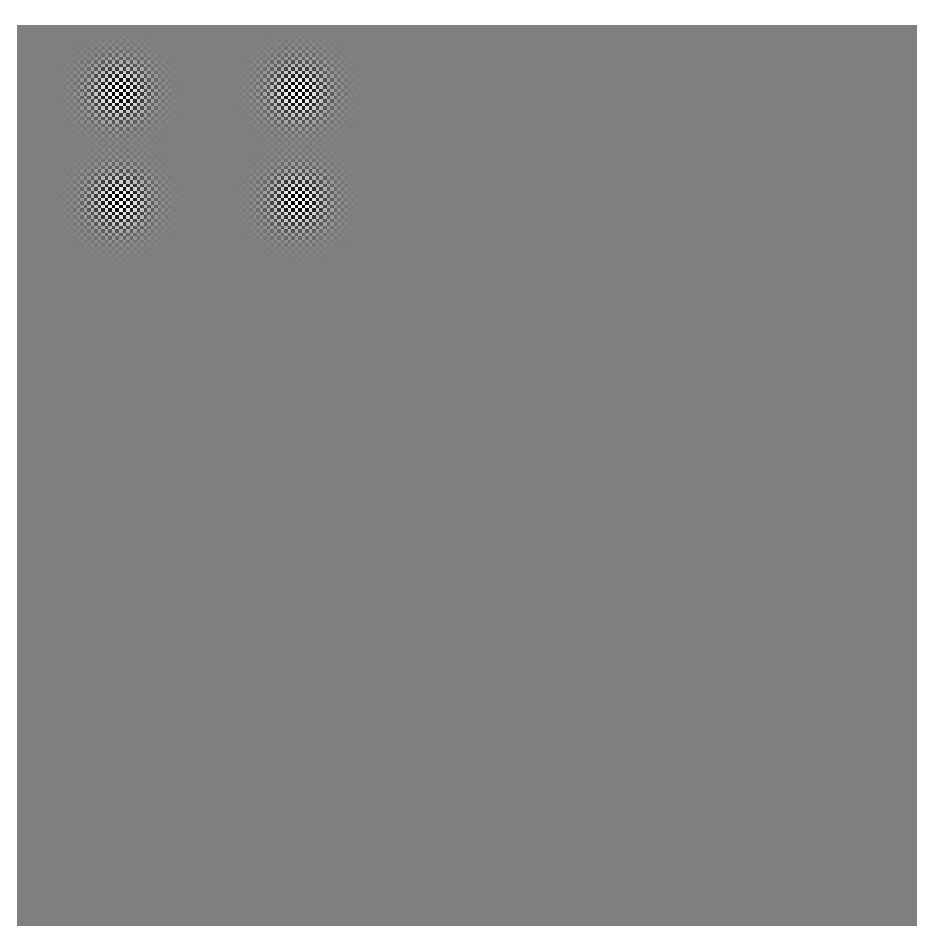
\includegraphics[width=0.5\textwidth]{figure/gradtest/Iout1}
\caption{发散的结果}\label{fig:Iout1}
\end{figure}
\begin{figure}[h!]
\center
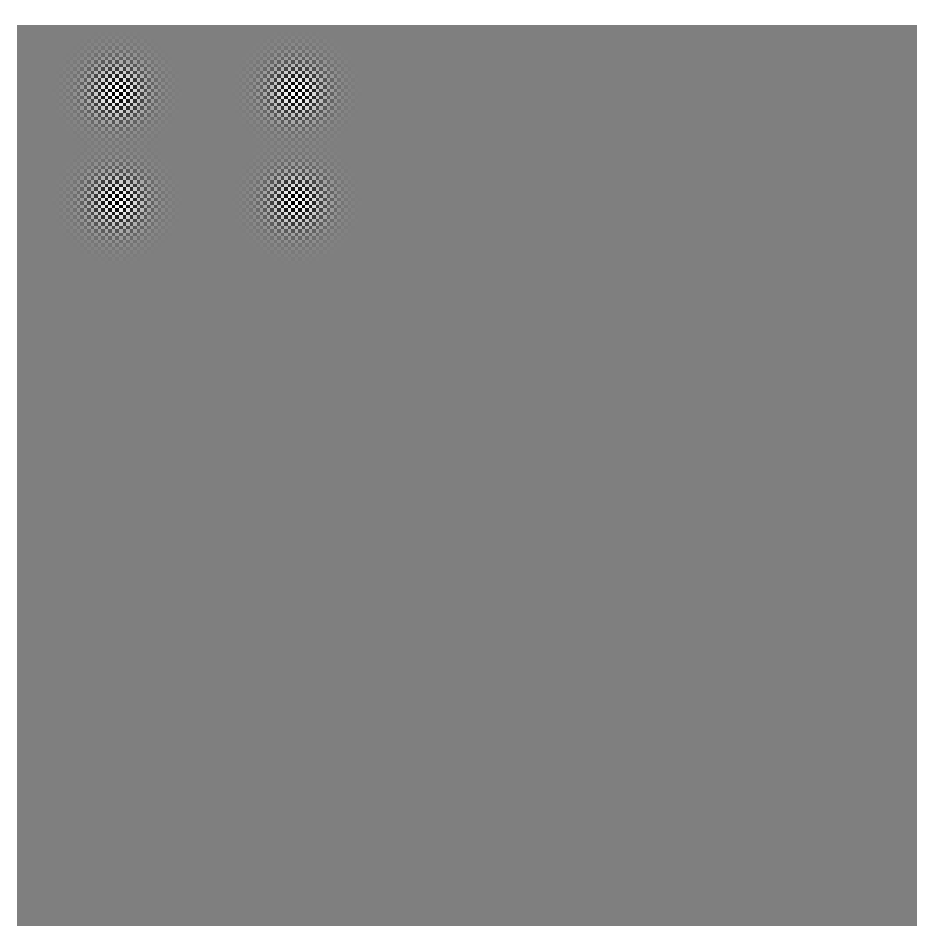
\includegraphics[width=0.5\textwidth]{figure/gradtest/Ioutx1}
\caption{发散的结果,x方向梯度}\label{fig:Ioutx1}
\end{figure}
\begin{figure}[h!]
\center
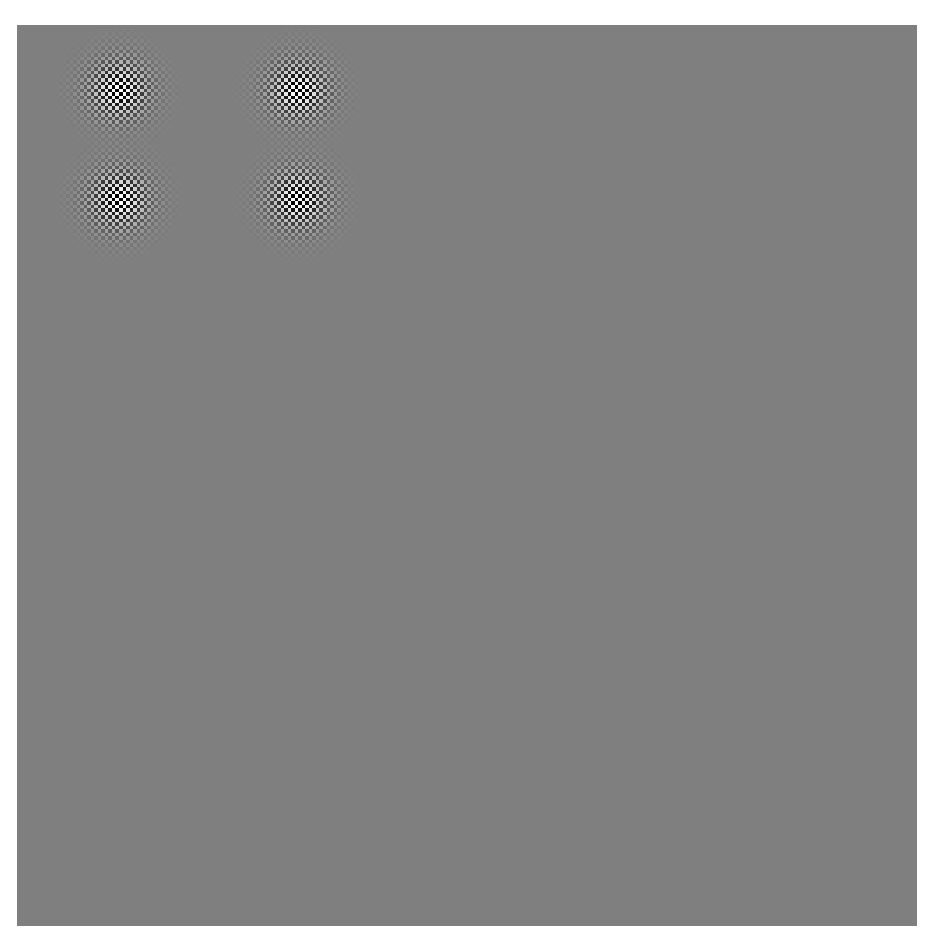
\includegraphics[width=0.5\textwidth]{figure/gradtest/Iouty1}
\caption{发散的结果,y方向梯度}\label{fig:Iouty1}
\end{figure}
可以发现两个方向的梯度与原图的纹理非常类似,也是没有什么意义的。事实上,当步进参数选择过大时,就会导致迭代中
的结果在最小值的周围来回震荡,或者直接发散开来,这与我们所得到的纹理图是想相类似的。
\FloatBarrier
\subsection{迭代次数}
如果我们选择一个合适的参数时,结果是收敛的。然而,如果迭代次数过少,会使得图像模板对原图的影响不平衡,
在接下来实验中选取了参数$\lambda=\xi=0.1$,并迭代30次。
\begin{figure}[h!]
\center
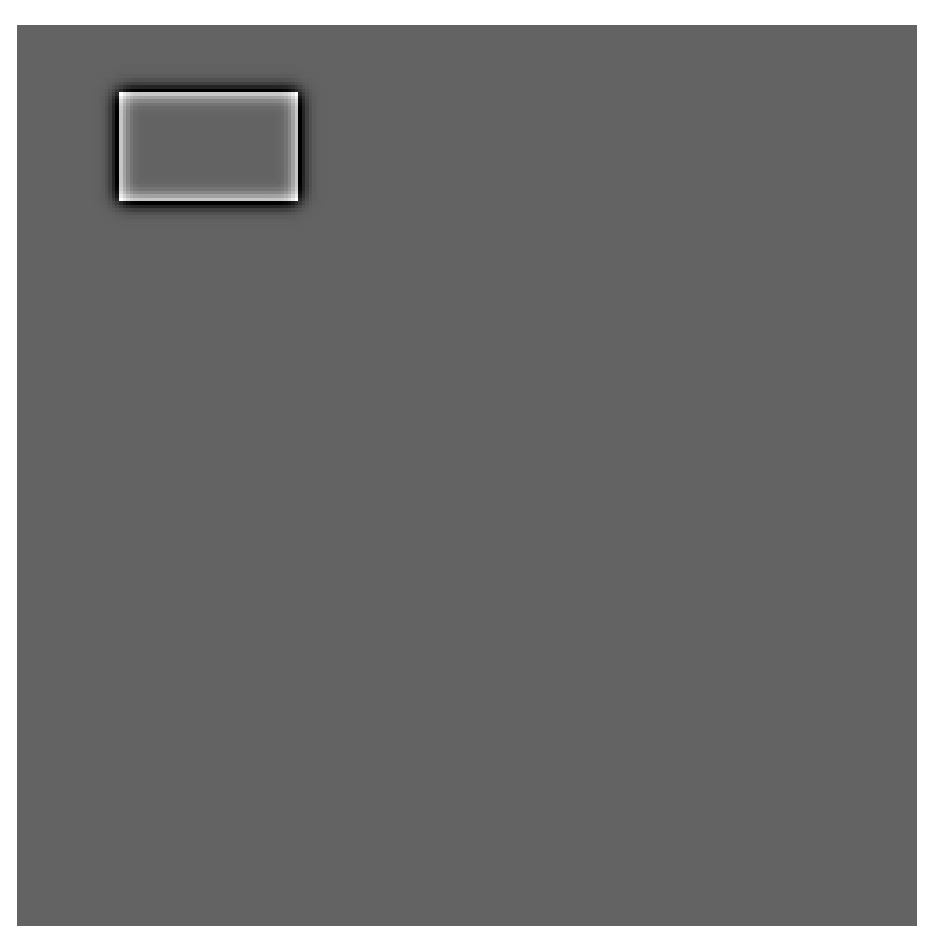
\includegraphics[width=0.5\textwidth]{figure/gradtest/Iout2}
\caption{$\lambda=\xi=0.1$,迭代次数30,结果}\label{fig:Iout2}
\end{figure}
\begin{figure}[h!]
\center
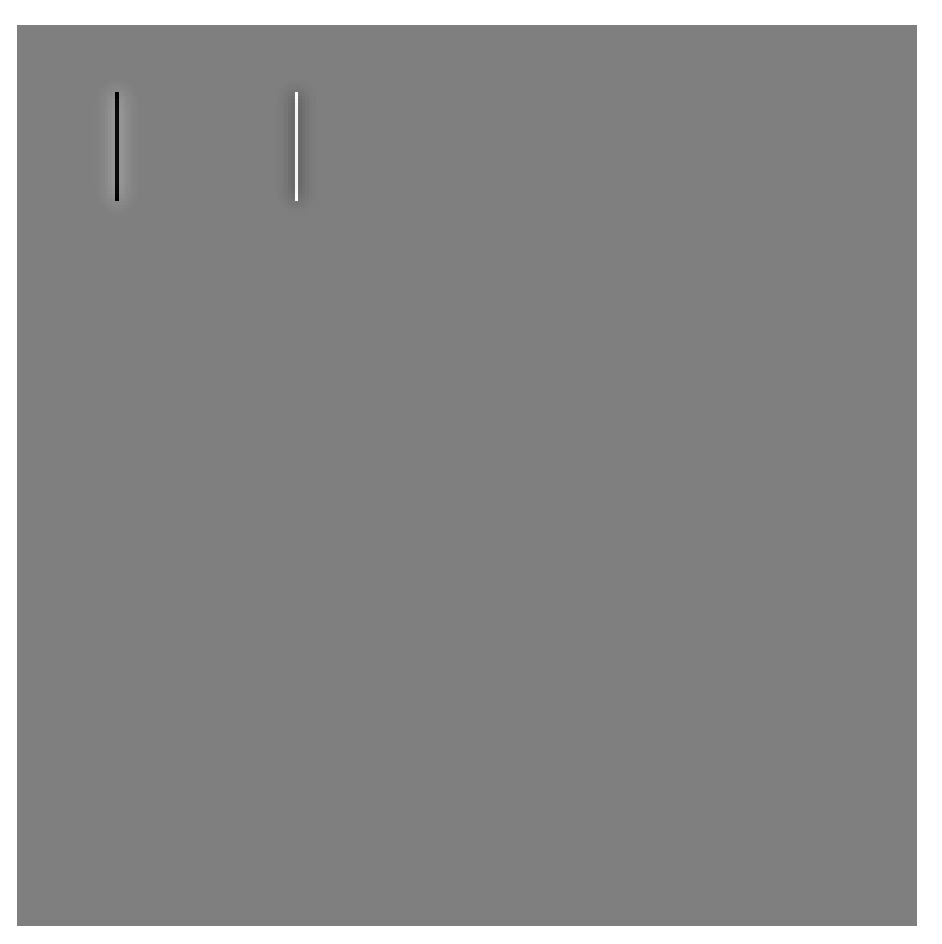
\includegraphics[width=0.5\textwidth]{figure/gradtest/Ioutx2}
\caption{$\lambda=\xi=0.1$,迭代次数30,x方向梯度}\label{fig:Ioutx2}
\end{figure}
\begin{figure}[h!]
\center
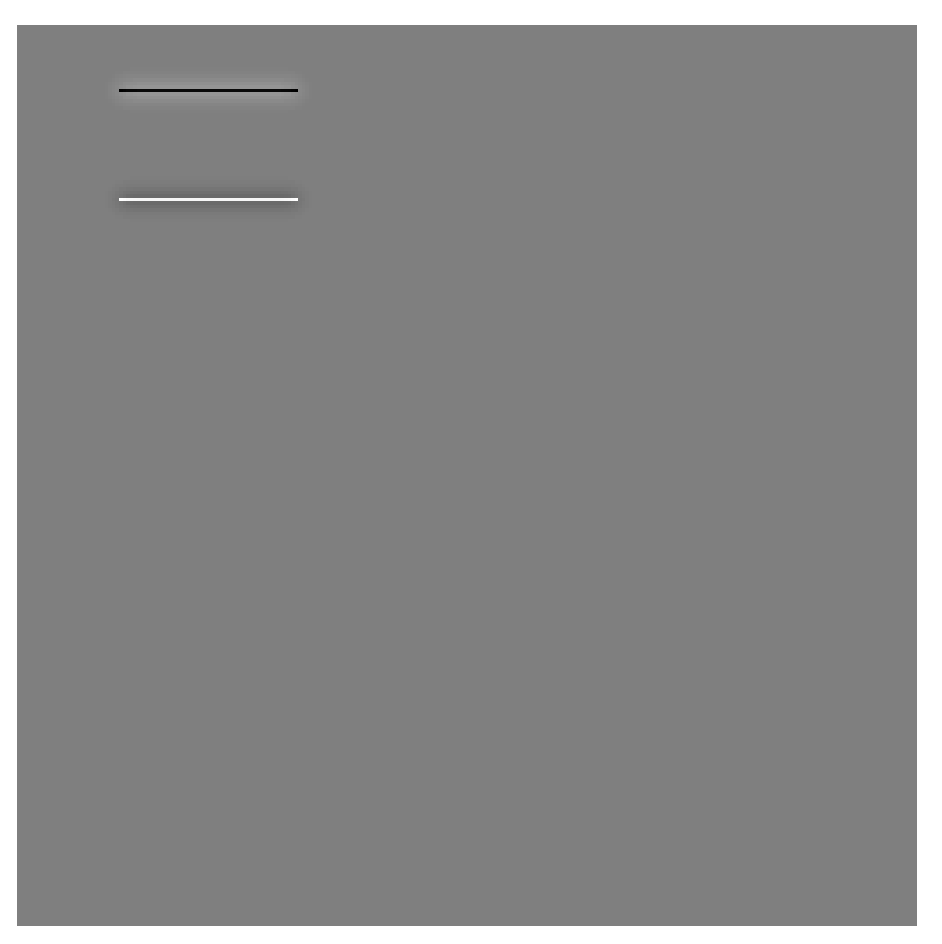
\includegraphics[width=0.5\textwidth]{figure/gradtest/Iouty2}
\caption{$\lambda=\xi=0.1$,迭代次数30,y方向梯度}\label{fig:Iouty2}
\end{figure}
图\ref{fig:Iout2}为相应结果图,图\ref{fig:Ioutx2}为$x$方向上的梯度,图\ref{fig:Iouty2}为$y$方向上的梯度。
从中可以看到梯度图像和梯度模板还是比较接近的,但是仍然有一些差距,反应到原图上,可以看到梯度模板对原图的
约束是从边缘处开始向内扩散的。因此迭代次数过少的时候,原图受到的影响并不平衡,比如方形内部受到的影响就
相对比较小。

\FloatBarrier
\subsection{合理的参数选择}
当参数选择合理得当的时候,该算法就可以取得较好的结果。在这里设置参数$\lambda=\xi=0.1$,迭代次数选择为$800$次。
所得到的结果,图\ref{fig:Iout3}为结果图像,图\ref{fig:Ioutx3}为$x$方向梯度图像,图\ref{fig:Iouty3}为$y$方向
梯度图像。
\begin{figure}[h!]
\center
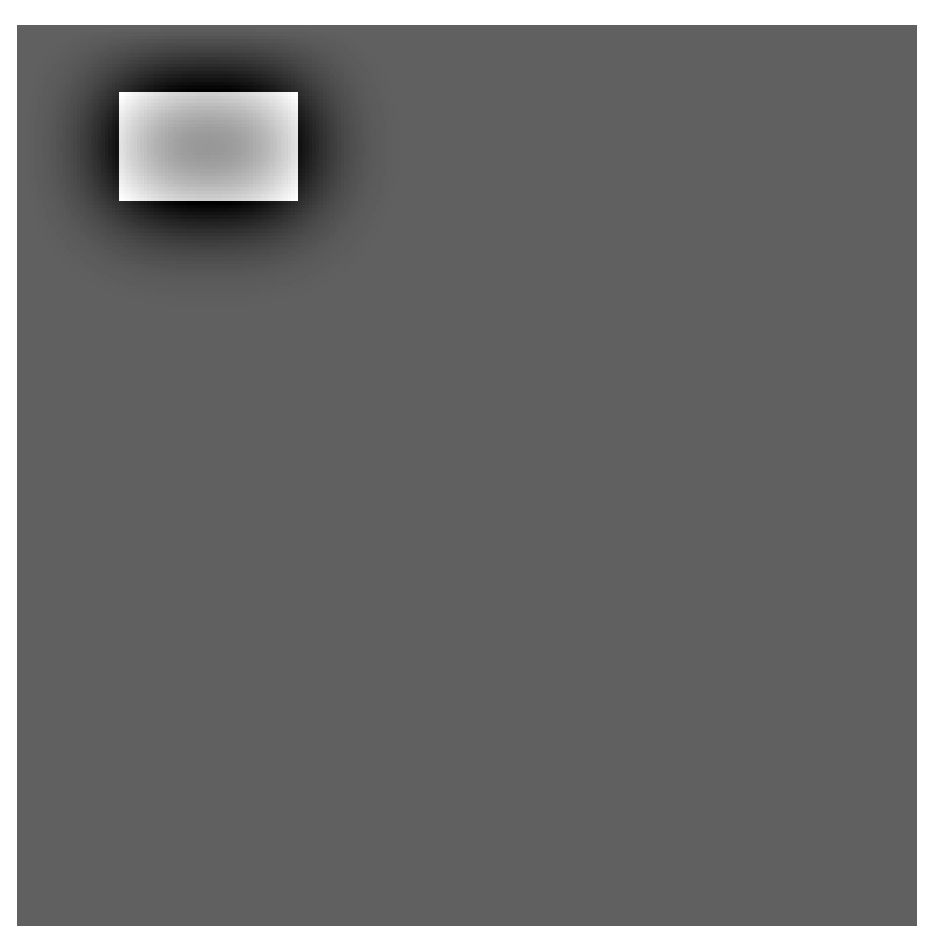
\includegraphics[width=0.5\textwidth]{figure/gradtest/Iout3}
\caption{$\lambda=\xi=0.1$,迭代次数800,结果}\label{fig:Iout3}
\end{figure}
\begin{figure}[h!]
\center
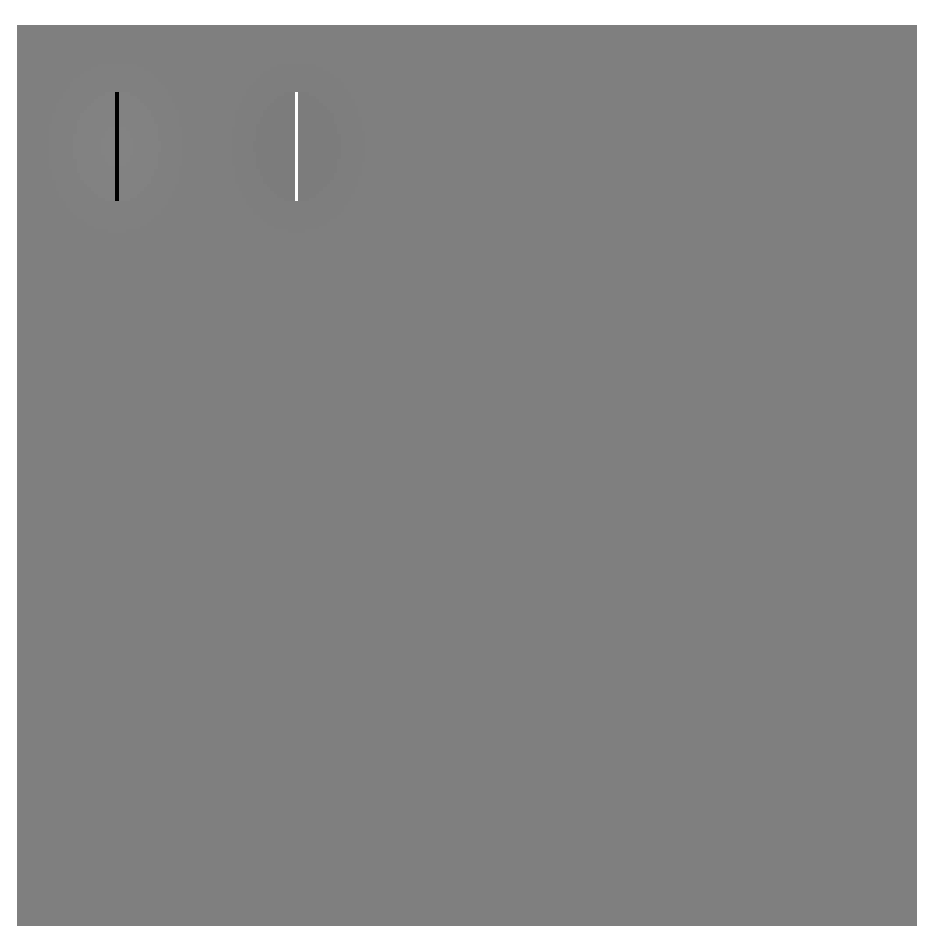
\includegraphics[width=0.5\textwidth]{figure/gradtest/Ioutx3}
\caption{$\lambda=\xi=0.1$,迭代次数800,x方向梯度}\label{fig:Ioutx3}
\end{figure}
\begin{figure}[h!]
\center
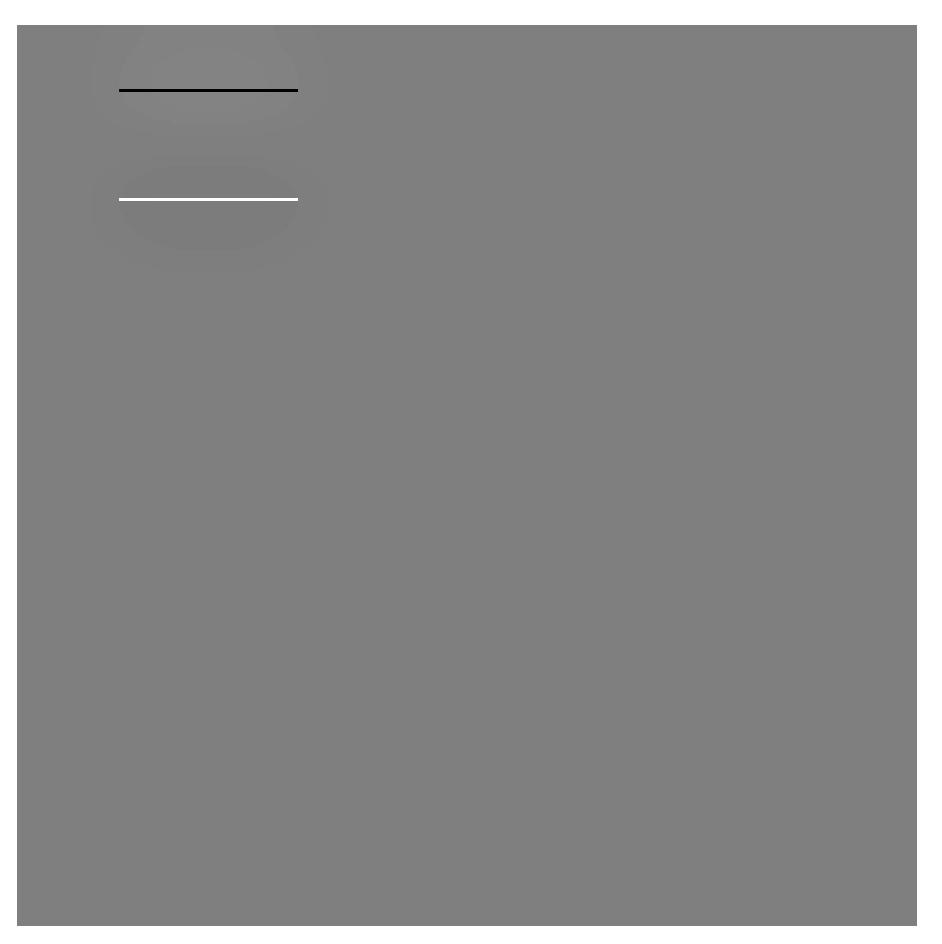
\includegraphics[width=0.5\textwidth]{figure/gradtest/Iouty3}
\caption{$\lambda=\xi=0.1$,迭代次数800,y方向梯度}\label{fig:Iouty3}
\end{figure}
可以看到,在迭代次数较大的情况下,结果图像的梯度与模板图像的梯度已经基本一致。而结果图由此也受到了影响,
可以发现在方形中间的部分也被模板图像所影响,使得中间部分的梯度趋于$0$。该算法的效果是明显的。

为了体现这个算法的另一种优势,即它并不会影响到原图的总体灰度分布,而只会在原图的基础上逐渐修改使得其梯度像
梯度图像靠拢,我们可以选择另一张图像作为原图。
\begin{figure}[h!]
\center
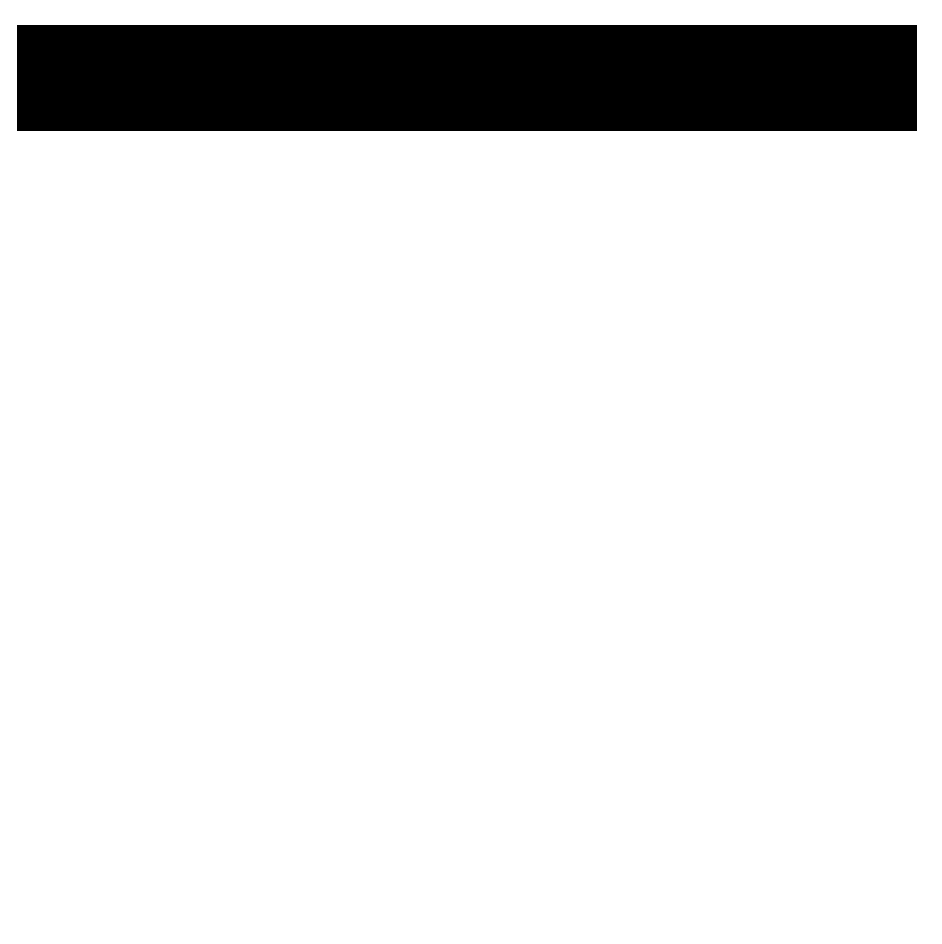
\includegraphics[width=0.5\textwidth]{figure/gradtest/I4}
\caption{用于测试灰度影响的原图}\label{fig:I4}
\end{figure}
\begin{figure}[h!]
\center
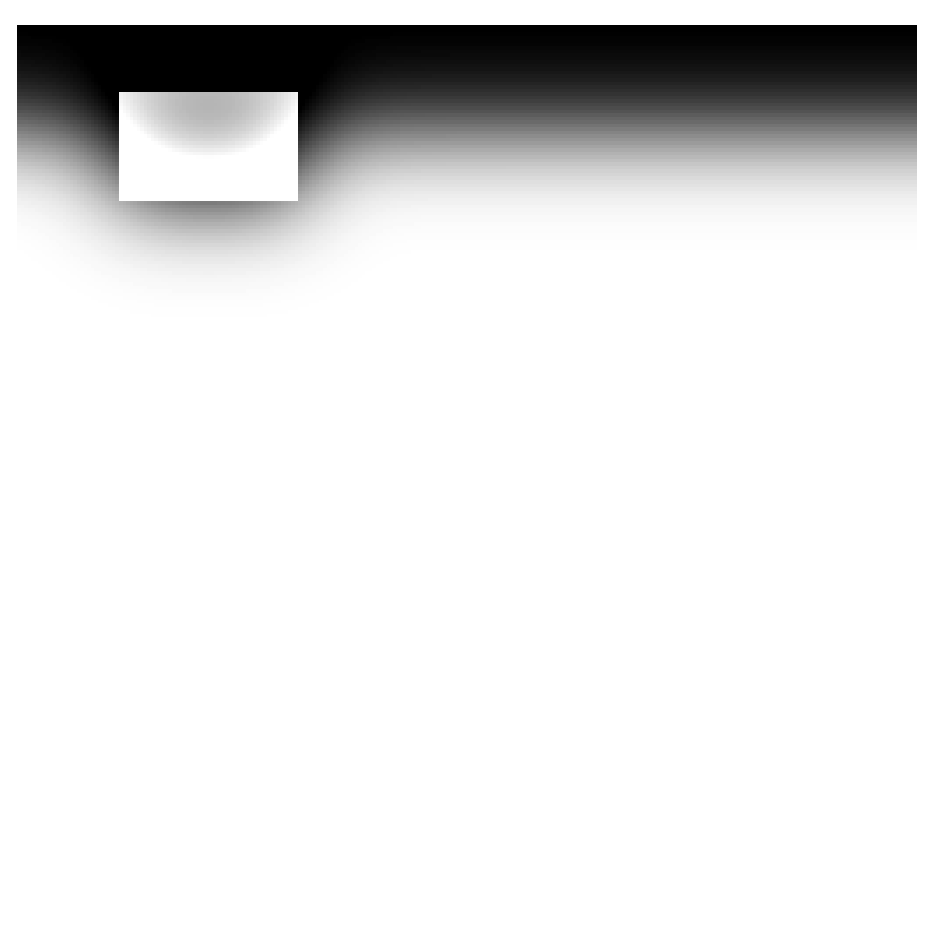
\includegraphics[width=0.5\textwidth]{figure/gradtest/Iout4}
\caption{迭代结果}\label{fig:Iout4}
\end{figure}
图\ref{fig:I4}是用于测试的原图。为了体现算法对灰度的影响,选取的原图大部分为白色,在应该是矩形的中部位置
有一条黑白分界线。这样,该图像大部分与梯度模板的灰度是反相的。

在该算法中,同样选取$\lambda=\xi=0.1$,迭代次数为$800$次,得到的结果图如图\ref{Iout4}所示。从这个结果图里,
我们可以看到,大部分的白色区域是没有受到影响的,而黑色区域也没有受到太多的影响。有影响的部分只有在梯度模板的
边缘与原图冲突的地方,其一是黑白交界处,由于此处在模板图像中梯度应该为$0$,所以可以看到此处的黑白交界被淡化了;
其二是矩形边缘,此处在模板图像中是有梯度边缘的,因此该处形成了矩形边缘,并向内扩散。

从上述的几个实验中,可以看到,只要相应的参数合理,并且迭代次数足够,梯度迭代项在实际使用中确实可以如理论一样
将模板图像的梯度信息融合到欲想要重建的图像中。

\section{梯度模板信息的处理}
为了能够提高重建的质量(包括重建后的被测物体清晰度以及降低噪声),我们需要从
超声数据中提取合理且有用的信息。正如前文所述,超声数据往往含有较多的噪声,
这些噪声不但会影响边界的提取,还会使得重建后的图像叠加上大量的噪声。

因此,对于超声数据如何处理,是一个比较重要的问题。这个处理过程包括降噪和去除无效斑块。
前者在超声数据原数据上作处理,而后者则在提取的梯度数据上进行处理。


\subsection{全变分降噪}
对于超声重建的原始数据,通常因为超声探测的原因,本身具备有不小的噪声。因此,第一步是
需要将图像进行降噪。经过测试,将使用全变分降噪(Total Variation Denoising)进行处理。

全变分降噪也成为全变分正则化(Total Variation Regularization),它
与简单的降噪,比如线性平滑(Linear Smoothing)相比,有着明显的优势。它可以明显
消除噪声,同时对边缘细节的破坏性比较小\cite{strong2003edge}。

全变分降噪是基于这样一个原理:对于一个有冗余细节以及噪声的图像,它的全变分值
往往很高,也就是说,它的梯度绝对值的积分很高。因此,需要寻找一个与原图相匹配且
全变分值相应较低的图像\cite{rudin1992nonlinear}。

在\cite{rudin1992nonlinear}中,二维图像全变分范数定义为
\begin{equation*}
V(y)=\sum_{i,j}\sqrt{|y_{i+1,j}-y_{i,j}|^2+|y_{i,j+1}-y_{i,j}|^2}
\end{equation*}
其中$y_{i,j}$为坐标为$i,j$的匹配图像像素。

但是一般采用更容易的形式
\begin{equation*}
V(y)=\sum_{i,j}|y_{i+1,j}-y_{i,j}|+|y_{i,j+1}-y_{i,j}|
\end{equation*}
采用最小平方误差来计算原图与匹配图像的误差,有
\begin{equation*}
E(x,y)=\cfrac{1}{2}\sum_{i,j}(x_{ij}-y_{ij})^2
\end{equation*}
其中$x$为原图像像素灰度。

于是全变分问题就变成了求解优化问题
\begin{equation*}
\min_yE(x,y)+\lambda V(y)
\end{equation*}

本文直接从网上下载了含有全变分降噪的工具箱来使用。
\begin{figure}[!h]\label{fig:beforeTV}
\center
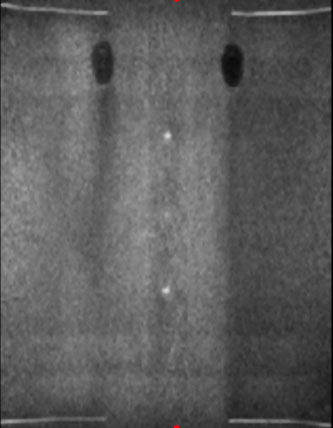
\includegraphics[width=0.7\textwidth]{figure/patternp/beforeTV.jpg}
\caption{全变分降噪前}
\end{figure}
\begin{figure}[!h]\label{fig:afterTV}
\center
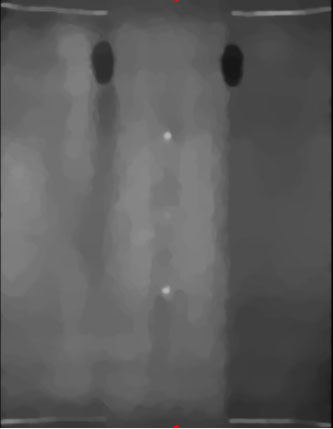
\includegraphics[width=0.7\textwidth]{figure/patternp/afterTV.jpg}
\caption{全变分降噪后}
\end{figure}
图\ref{fig:beforeTV}为全变分降噪之前的原始数据,而图\ref{fig:afterTV}为全变分降噪之后。
对比两图,可以发现,正如全变分降噪理论上的特点,噪声被很好地消除,同时,边缘细节并
没有被模糊。


\subsection{梯度数据修正}
对于降噪之后的图像,本文通过梯度运算直接求得其梯度图像。但是,这个梯度图像是存在瑕疵的。
主要问题是边缘毛刺大,且边缘不够平滑,此外,还存在不属于有效信息的小斑块\footnote{我们考虑
到这可能是全变分降噪算法的一些不良影响}。因此,需要让梯度数据经过一系列处理,得到更合理
的梯度数据。这种处理,也可以理解为我们从超声数据中提取有用信息的一部分。处理过程示意如下:
\begin{equation*}
\boxed{\text{降噪后噪声数据}}\xlongrightarrow{提取梯度}
\boxed{\text{梯度数据}}\xlongrightarrow{灰度开运算}
\boxed{\text{去斑块后数据}}\xlongrightarrow{中值滤波}
\boxed{\text{噪声降低}}\xlongrightarrow{灰度腐蚀膨胀}
\boxed{\text{最终结果}}
\end{equation*}
\begin{enumerate}
\item 灰度开运算

灰度开运算是灰度腐蚀和灰度膨胀的连续运算。灰度开运算因为先腐蚀,会消除掉较小的斑块。而腐蚀和
膨胀的连续运算,可以使得整体的形态和亮度维持不变。因此,灰度开运算可以有效去除
无效的亮点信息。

\item 中值滤波

为了进一步去除噪点,在灰度开运算之后,还使用了一次中值滤波。中值滤波通过设置一个像素
点为其邻域窗口内的中位数点,可以有效消除和平滑掉较小的噪点。相对于直接平滑,它对
图像结构的破坏性也比较低。

\item 灰度腐蚀与膨胀

同样,由于采用全变分降噪的原因,梯度图像里得到的有效边缘往往比较粗,这对于重建是不利的。
由于梯度具有正梯度值和负梯度值,需要将之分别采用灰度腐蚀与灰度膨胀进行处理,细化梯度边缘。
灰度腐蚀可以让灰度值高的边缘处降低灰度,并向中心靠齐,而灰度膨胀则让边缘处的灰度上升,对于
负梯度而言,起到的效果与灰度腐蚀在正梯度处效果是一致的。
\end{enumerate}

考虑到所提取的梯度有$x$,$z$两个方向,也就两组数据,本文分别在两组方向上的每一个平面进行上面
的处理过程。也就是说,对于$x$方向的梯度,则在与$x$轴垂直的每层平面上作相应的处理;对于$z$方向
的梯度,则在与$z$轴垂直的每层平面上作处理。
\begin{figure}[!h]\label{fig:afterTV}
\center
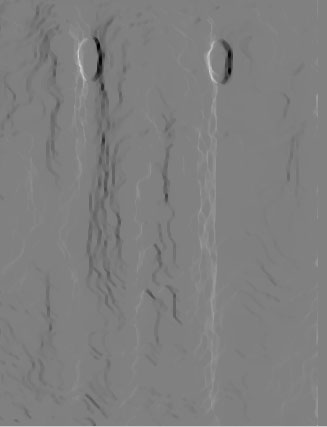
\includegraphics[width=0.7\textwidth]{figure/patternp/gradp.jpg}
\caption{修正后梯度}
\end{figure}
图\ref{fig:gradp}是沿着与$x$方向相垂直的视点所看进去而截取的一片截面,也是图\ref{fig:afterTV}
通过了梯度截取以及处理之后的图像。可以看到,在这个截面中,梯度
信息已经十分清晰,且基本没有噪点。

在最后的实验效果中也证明了,这种处理方法的效果是很好的,提取出来的信息对重建的帮助也很大。


\section{SART迭代项A矩阵的获得}
在章节\ref{sec:sartA}中,已经详细描述了在二维平面的投影矩阵获得方法。在本文所实验用的
模型是一个三维模型,投影矩阵的获得需要作一些改动,当然,基本是类似的。

考虑到探测光束将从物体的上方以不同的角度和位置穿过物体,其有一段将与物体直接相交。根据
\ref{sec:sartA}所提到的方式,需要将相交的这段线段等分。每个等分点的灰度值由周围的八个顶点
来决定,因此需要对此进行三维的插值。在投影矩阵中,需要因此来计算插值系数。与二维的双线性插值类似,
采用三线性插值。相邻八个顶点上的的插值系数可以采用下面公式计算:
\begin{equation}
c = \cfrac{l_1l_2l_3}{h_1h_2h_3}
\end{equation}
其中,$c$为插值系数,$l_1,l_2,l_3$分别为被插值点坐标到在插值立方体内以该顶点为顶点的三个面的距离,
而$h_1,h_2,h_3$则为与对应距离平行的立方体的边长值。

每一个像素点上的插值系数,由这束光每个点所产生的插值系数叠加并乘上等分补偿得到。从公式\eqref{eq:computea}可以得到:
\begin{equation}\label{eq:computea}
a_{ij}=\sum^{M_j}_{m=1}c_{ijm}\Delta s
\end{equation}

这里在等分步长的选择上,按照章节\ref{sec:sartA}所提到的,采用采样长度的一半。

\section{迭代方式修正}
在实际实验中,投影迭代项的计算需要花费大量的时间,且其收敛速度比较快;而相比较,
梯度迭代项的计算时间短,但是需要迭代较多次才能收敛。因此,迭代公式\eqref{eq:all}并不是直接被使用的。

考虑到迭代公式的每个迭代项都有一个迭代步长系数,而实际上这个补偿系数是不需要固定的。在一些迭代中,如果
我们设置投影迭代项的步长为$0$,那么实际上在这次迭代中投影数据不参与迭代,也就不需要计算一次投影数据。
这样,就相当于少部分迭代有投影数据的参与,而大部分迭代只有梯度数据,这样,就可以解决两者收敛情况不一致的
矛盾。从变步长梯度下降的角度看,这样的迭代方式改进也是合理的。

在实验中,有$21$个不同角度的投影,且总的迭代轮数为$3$轮。因此,采用的迭代次数是投影数据迭代次数为$21*3$,而不含有
投影数据的迭代次数为其$15$倍,也就是$21*3*15$。

经过测试,这样的迭代次数是合理的,能够让CT重建和梯度信息融合这两种过程都达到一个较好的结果。

\section{代码实现}
在最终试验测试中,主要采用Matlab和C程序共同运行的方式。其中,Matlab主要用来负责超声数据的
处理过程,包括配准,全变分降噪,提取梯度,以及梯度修正等等,并将之存储为可以被C
程序所识别的数据形式。而C程序由于其高效的特性,被用于计算量最大的重建部分。重建部分也是
代码实现最重要的部分,以下将作一些详细介绍。

\subsection{模型参数}
由于系统在几何上有较多的信息,因此,模型所具有的参数也较为繁多。见表\ref{tab:para}。
\begin{table}[!h]\label{tab:para}
\center
\caption{模型参数}
\vspace{1pc}
\begin{tabular}{r|l}
\hline
参数        &     大小\\
\hline
探测面长     &   1152   \\
\hline
探测面宽    &     580 \\
\hline  
重建区域长   &   1008 \\
\hline 
重建区域宽  &  524 \\
\hline   
重建区域底面高度  &   157  \\
\hline
重建区域顶面高度  &   372   \\
\hline 
重建区域纵向层数  &  430   \\
\hline
投影组数       &  21 \\
\hline
\end{tabular}
\end{table}
\subsection{数据的存储与导入}
实验中会涉及到大量数据的处理,包括投影数据以及超声数据。

对于投影数据,是以dat格式存储,每个数据以浮点格式存储在文件内,通过C代码可以直接
读取和导入。而对于超声数据,原始是以tif格式存储。在实验中,使用Matlab将之读取,
并经过处理之后,将之存储为dat格式供C程序读取。
\subsection{投影矩阵获得}
投影矩阵的获得是C程序中很重要的部分之一,其步骤主要如下:
\begin{enumerate}
\item 根据每一个投影点计算对应的光束的直线方程参数。
\item 确定参数之后,判断每一条光束与重建区域在哪些边缘平面相交。并根据结果,确定每一条光束与重建区域的边缘交点。
\item 根据边缘交点,在光束上找到每一个等分点位置,并根据等分点坐标,以方程\eqref{eq:computed}来计算插值系数。
\item 对每一条光束作同样计算,就可以得到投影矩阵。
\end{enumerate}
\subsection{稀疏矩阵存储}
实际上,分析投影矩阵,可以发现,对于一条光束$j$,元素$a_{ij}$只有在光束经过的地方附近的点才具有插值系数,别的则为$0$。
而这与整个重建区域的体素相比,是非常稀少的。因此,投影矩阵可以采用稀疏矩阵存储。

如果只是按照普通的矩阵存储,则需要花费的空间是很大的。如果将其以稀疏矩阵方式存储,则在读取时
只会少花费一点时间,但是可以节约大量的内存。因此,在C程序代码中,每次计算出一条光束的
插值系数,就将之存储到稀疏矩阵的数据结构之中。
\section{算法结果}
在使用基于SART的优化算法之前,我们将投影数据按照SART的方式直接重建一次,这次重建不包含
任何先验知识。选取一些结果如图\ref{fig:origin1}-\ref{fig:origin4}所示。
\begin{figure}[!ht]\label{fig:origin1}
\center
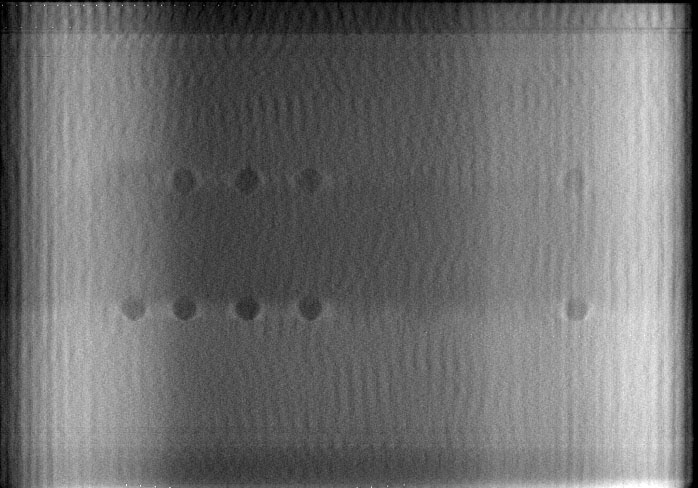
\includegraphics[width=0.6\textwidth]{figure/result/origin1.jpg}
\caption{直接CT重建截面1}
\end{figure}
\begin{figure}[!ht]\label{fig:origin2}
\center
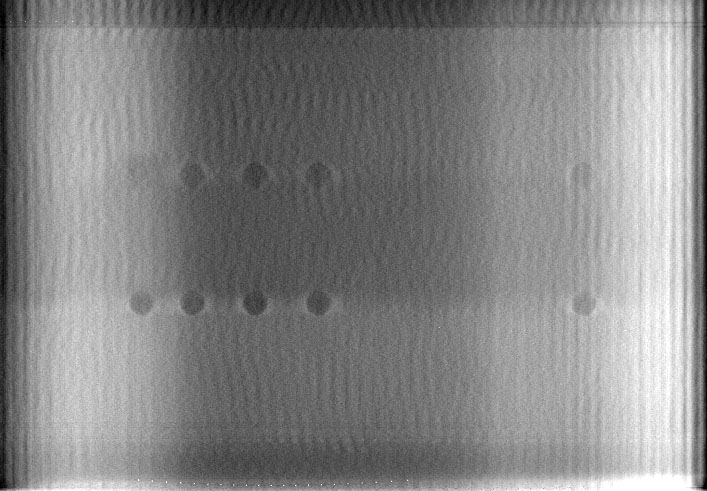
\includegraphics[width=0.6\textwidth]{figure/result/origin2.jpg}
\caption{直接CT重建截面2}
\end{figure}
\begin{figure}[!ht]\label{fig:origin3}
\center
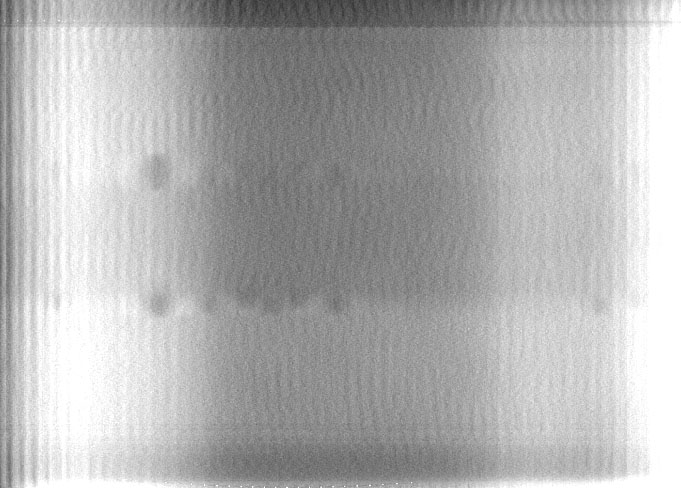
\includegraphics[width=0.6\textwidth]{figure/result/origin3.jpg}
\caption{直接CT重建截面3}
\end{figure}
\begin{figure}[!ht]\label{fig:origin4}
\center
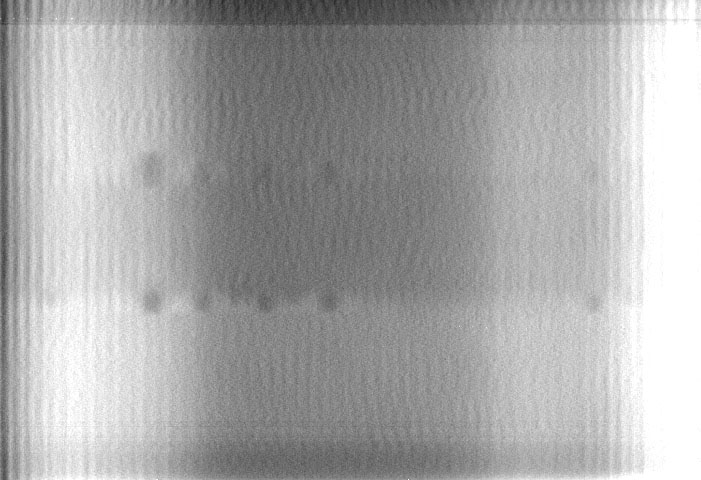
\includegraphics[width=0.6\textwidth]{figure/result/origin4.jpg}
\caption{直接CT重建截面4}
\end{figure}

从图中可以看到,由于有限角度CT成像的原因,图中的肿块边缘在随着物体深度变化时,
并没有明显的变化,而是逐渐模糊消失的。且图\ref{fig:origin4}已经到了肿块应该
完全消失的深度,但是却依然能看到肿块模糊的影子。这种情况是十分不利于CT重建结果的应用的。

在边缘的变化上,超声数据有着明显的优势。见图\ref{fig:us1}-\ref{fig:us4}
\begin{figure}[!ht]\label{fig:us1}
\center
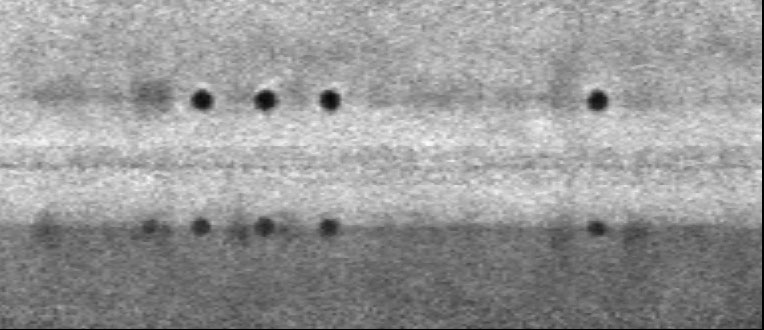
\includegraphics[width=0.6\textwidth]{figure/result/us1.jpg}
\caption{超声数据截面1}
\end{figure}
\begin{figure}[!ht]\label{fig:us2}
\center
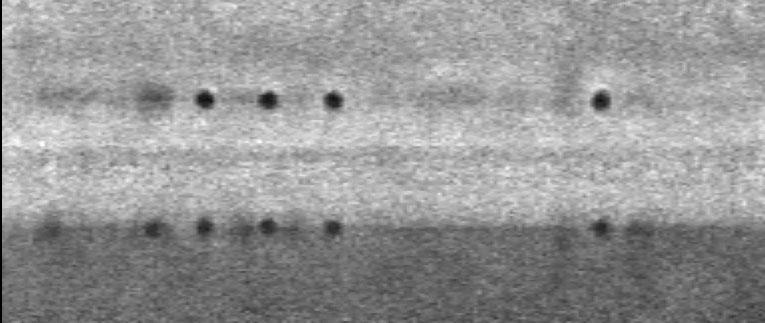
\includegraphics[width=0.6\textwidth]{figure/result/us2.jpg}
\caption{超声数据截面2}
\end{figure}
\begin{figure}[!ht]\label{fig:us3}
\center
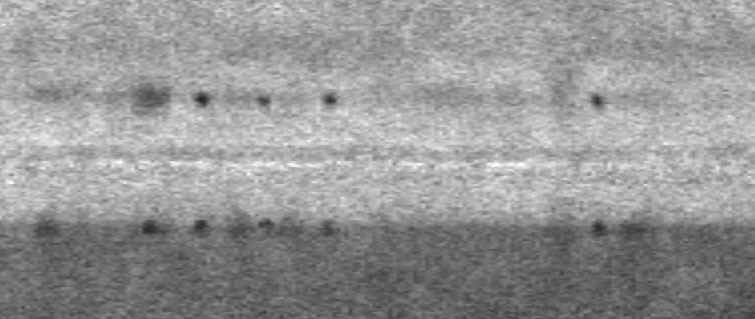
\includegraphics[width=0.6\textwidth]{figure/result/us3.jpg}
\caption{超声数据截面3}
\end{figure}
\begin{figure}[!ht]\label{fig:us4}
\center
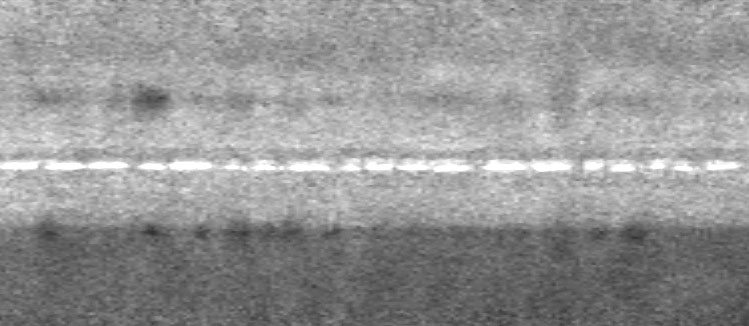
\includegraphics[width=0.6\textwidth]{figure/result/us4.jpg}
\caption{超声数据截面4}
\end{figure}
从图中可以看到,超声数据边缘的变化是十分明显的,与同样深度的原始CT重建相比。然而超声数据
有两点劣势可以直接从图中看到。首先,超声数据的分辨率相比TOMO是很低的,此外,超声数据的噪声
十分严重。

在使用了基于SART的优化算法来重建CT图像,其产生的结果如图\ref{fig:final1}-\ref{fig:final4}:
\begin{figure}[!ht]\label{fig:final1}
\center
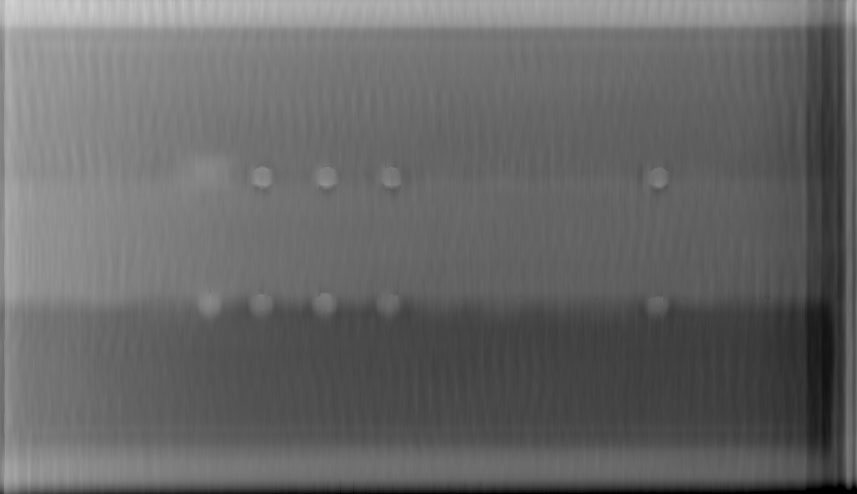
\includegraphics[width=0.6\textwidth]{figure/result/final1.jpg}
\caption{优化的CT重建1}
\end{figure}
\begin{figure}[!ht]\label{fig:final2}
\center
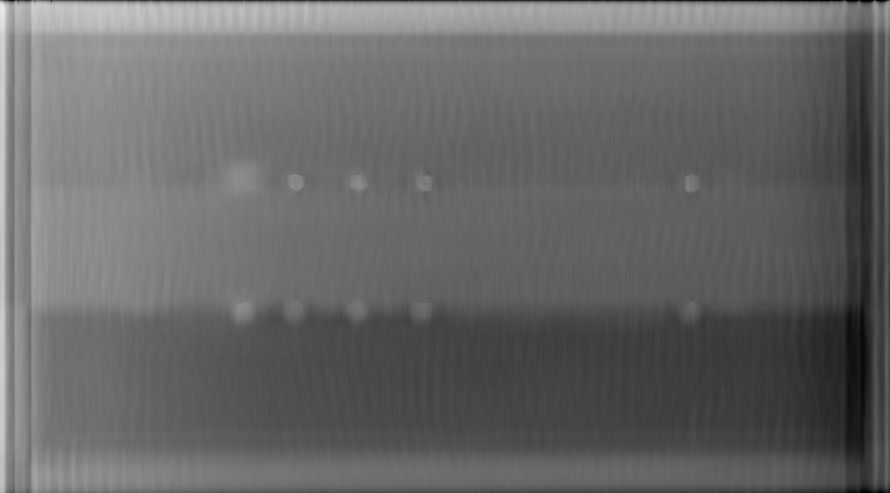
\includegraphics[width=0.6\textwidth]{figure/result/final2.jpg}
\caption{优化的CT重建2}
\end{figure}
\begin{figure}[!ht]\label{fig:final3}
\center
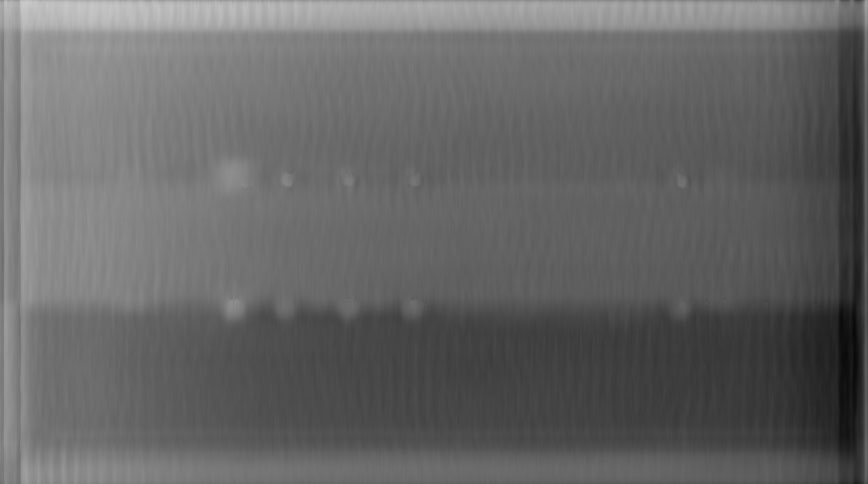
\includegraphics[width=0.6\textwidth]{figure/result/final3.jpg}
\caption{优化的CT重建3}
\end{figure}
\begin{figure}[!ht]\label{fig:final4}
\center
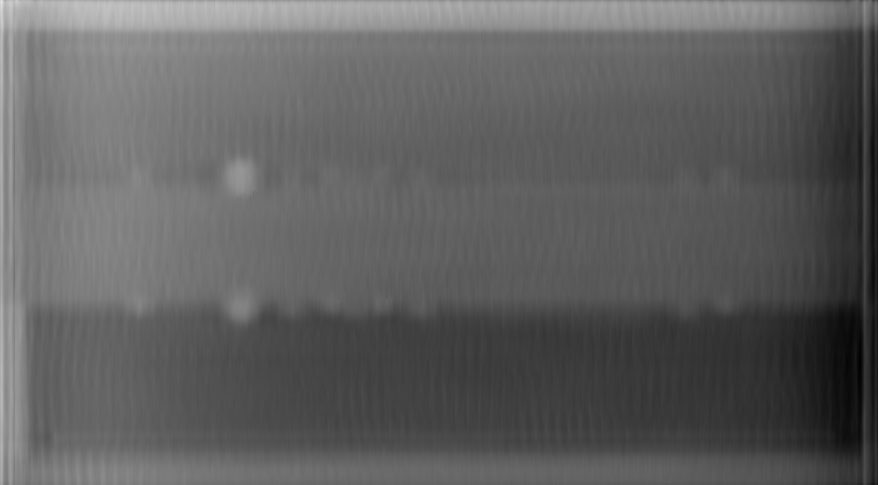
\includegraphics[width=0.6\textwidth]{figure/result/final4.jpg}
\caption{优化的CT重建4}
\end{figure}
由于计算的原因,图像的颜色相反。此外,由于超声图像对其中一个
肿块的探测很差,因此相应的肿块就没有被优化到。
对比相应的超声图像和原始CT重建图像,可以看到,
优化后的CT重建具备了上述两个图像的优点。对比同样深度的优化CT图像和
原始CT图像,优化后的CT图像在边缘上出现了
明显的变化,边缘也更加清晰易见。

在提高了CT图像重建的边缘变化清晰度的同时,优化CT重建所检测到的探测物体内部
的分层(可以看到图中有三个不同的层次)并没有因为超声图像相反的
颜色特性而被破坏掉。而很明显地,优化后的CT重建同样保留了CT图像噪声小、分辨率高的
优点。

注意到变小的肿块后方还有一层重影,这是因为本文所使用的迭代方式所致的,因为两种迭代项
有很多次是分开迭代的,因此会造成重建出来的图像含有原始CT重建的影子。如果两者的同时迭代
且次数较多,可以解决此问题,但是考虑到时间成本,就没有实行此方案。
\section{小结}
本章节主要是对提出的算法进行了验证,也解决了本文所要研究的探测模型问题。

对于提出的基于SART的优化算法,本章先是在不适用投影约束的情况下,用玩具模型测试了
使用梯度信息作为约束的优化算法的可行性,并对使用的参数有了一个大概范围的估计。从实验中,
可以看出,需要合理选择迭代的步进大小与迭代次数,才可以达到一个效率与精确度平衡。

接下来讨论了本算法在具体问题上实施所需要的细节,包括三维情况下投影矩阵的获得,
迭代次数的修改,以及在代码上所使用的语言与数据结构等等。

在最后,给出了原始CT重建、超声数据以及优化后CT重建结果在同一层下的对比。可以很清楚看到,
基于SART的优化算法有效改进了CT重建的边缘模糊不清问题,同时又保留了CT重建的高分辨率以及
低噪声的优势,从而看出,该算法是完全可行的。
\bibliography{thesis}
\chapter{致谢}
\end{document}



